%% USPSC-TCC-modelo.tex
% ---------------------------------------------------------------
% USPSC: Modelo de Trabalho Academico (tese de doutorado, dissertacao de
% mestrado e trabalhos monograficos em geral) em conformidade com
% ABNT NBR 14724:2011: Informacao e documentacao - Trabalhos academicos -
% Apresentacao
%----------------------------------------------------------------
%% Esta é uma customização do abntex2-modelo-trabalho-academico.tex de v-1.9.5 laurocesar
%% para as Unidades do Campus USP de São Carlos:
%% EESC - Escola de Engenharia de São Carlos
%% IAU - Instituto de Arquitetura e Urbanismo
%% ICMC - Instituto de Ciências Matemáticas e de Computação
%% IFSC - Instituto de Física de São Carlos
%% IQSC - Instituto de Química de São Carlos
%%
%% Este trabalho utiliza a classe USPSC.cls que é mantida pela seguinte equipe:
%%
%% Coordenação e Programação:
%%   - Marilza Aparecida Rodrigues Tognetti - marilza@sc.usp.br (PUSP-SC)
%%   - Ana Paula Aparecida Calabrez - aninha@sc.usp.br (PUSP-SC)
%% Normalização:
%%   - Brianda de Oliveira Ordonho Sigolo - brianda@usp.br (IAU)
%%   - Eduardo Graziosi Silva - edu.gs@sc.usp.br (EESC)
%%   - Eliana de Cássia Aquareli Cordeiro - eliana@iqsc.usp.br (IQSC)
%%   - Flávia Helena Cassin - cassinp@sc.usp.br (EESC)
%%   - Maria Cristina Cavarette Dziabas - mcdziaba@ifsc.usp.br (IFSC)
%%   - Regina Célia Vidal Medeiros - rcvmat@icmc.usp.br (ICMC)
%%
%% O USPSC-modelo.tex e USPSC-TCC-modelo.tex utilizam diversos arquivos relacionado em
%% 2.1 Pacote USPSC: Classe USPSC e modelos de trabalhos acadêmicos	do Tutorial do Pascote
%%  USPSC para modelos de trabalhos de acadêmicos em LaTeX - versão 3.1


%----------------------------------------------------------------
%% Sobre a classe abntex2.cls:
%% abntex2.cls, v-1.9.5 laurocesar
%% Copyright 2012-2015 by abnTeX2 group at https://www.abntex.net.br/
%%
%----------------------------------------------------------------

\documentclass[
% -- opções da classe memoir --
12pt,		% tamanho da fonte
openright,	% capítulos começam em pág ímpar (insere página vazia caso preciso)
oneside,  % para impressão em anverso (frente) e verso. Oposto a oneside - Nota: utilizar \imprimirfolhaderosto*
%oneside, % para impressão em páginas separadas (somente anverso) -  Nota: utilizar \imprimirfolhaderosto
% inclua uma % antes do comando twoside e exclua a % antes do oneside
a4paper,			% tamanho do papel.
% -- opções da classe abntex2 --
chapter=TITLE,		% títulos de capítulos convertidos em letras maiúsculas
% -- opções do pacote babel --
english,			% idioma adicional para hifenização
french,				% idioma adicional para hifenização
spanish,			% idioma adicional para hifenização
brazil				% o último idioma é o principal do documento
% {USPSC-classe/USPSC} configura o cabeçalho contendo apenas o número da página
]{USPSC-classe/USPSC}
%]{USPSC-classe/USPSC1}
% Inclua % antes de ]{USPSC-classe/USPSC} e retire a % antes de %]{USPSC-classe/USPSC1} para utilizar o
% cabeçalho diferenciado para as páginas pares e ímpares:
%- páginas ímpares: com seções ou subseções e o número da página
%- páginas pares: com o número da página e o título do capítulo
% ---
% ---
% Pacotes básicos - Fundamentais
% ---
\usepackage[T1]{fontenc}		% Seleção de códigos de fonte.
\usepackage[utf8]{inputenc}		% Codificação do documento (conversão automática dos acentos)
\usepackage{lmodern}			% Usa a fonte Latin Modern
% Para utilizar a fonte Times New Roman, inclua uma % no início do comando acima  "\usepackage{lmodern}"
% Abaixo, tire a % antes do comando  \usepackage{times}
%\usepackage{times}		    	% Usa a fonte Times New Roman
% Para usar a fonte , lembre-se de tirar a % do comando %\renewcommand{\ABNTEXchapterfont}{\rmfamily}, localizado mais abaixo, logo após "Outras opções para nota de rodapé no Sistema Numérico"
\usepackage{lastpage}			% Usado pela Ficha catalográfica
\usepackage{indentfirst}		% Indenta o primeiro parágrafo de cada seção.
\usepackage{color}				% Controle das cores
\usepackage{graphicx}			% Inclusão de gráficos
\usepackage{float} 				% Fixa tabelas e figuras no local exato
\usepackage{chemfig,chemmacros} % Para escrever reações químicas
\usepackage{tikz}				% Para escrever reações químicas e outros
\usetikzlibrary{positioning}
\usepackage{microtype} 			% para melhorias de justificação
\usepackage{pdfpages}
\usepackage{makeidx}            % para gerar índice remissivo
\usepackage{hyphenat}          % Pacote para retirar a hifenizacao do texto
\usepackage[absolute]{textpos} % Pacote permite o posicionamento do texto
\usepackage{eso-pic}           % Pacote para incluir imagem de fundo
\usepackage{makebox}           % Pacote para criar caixa de texto

\usepackage{graphicx}
\usepackage{graphbox}
\usepackage{tasks}
\usepackage{amssymb}
\usepackage{amsmath}
\usepackage{amsthm}
\usepackage{fontawesome5}

% TODO List
\usepackage{todonotes}

\usepackage{svg} % ADDED JORGE FOR SVG

\usepackage[ruled]{algorithm2e}

\usepackage{tikz}
\usepackage{aircraftshapes}

\usetikzlibrary{positioning}

\newcommand{\destaq}[1]{\textcolor{BlueViolet}{\textbf{#1}}}
\renewcommand\todo[1]{\colorbox{green}{#1}}

\definecolor{echodrk}{HTML}{0099cc}
\definecolor{olivegreen}{rgb}{0,0.6,0}
\definecolor{camdrk}{RGB}{0,62,114}

\usetikzlibrary{arrows,shapes}

\definecolor{mygreen}{rgb}{0,0.6,0}

\definecolor{mymauve}{rgb}{0.58,0,0.82}

\usetikzlibrary{arrows,shapes, decorations.pathmorphing,backgrounds,positioning}

\pgfdeclarelayer{background}
\pgfsetlayers{background,main}

\tikzstyle{vertex}=[circle,fill=black!25,minimum size=20pt,inner sep=0pt]
\tikzstyle{selected vertex} = [vertex, fill=red!24]
\tikzstyle{select vertex} = [vertex, fill=blue!24]
\tikzstyle{selectx vertex} = [vertex, fill=green!24]
\tikzstyle{edge} = [draw,thick,-]
\tikzstyle{selected edge} = [draw,line width=5pt,-,red!50]

\usepackage{minted}
\usemintedstyle{vs}

\usepackage{enumitem}
\newlist{todolist}{itemize}{2}
\setlist[todolist]{label=$\square$}
\usepackage{pifont}
\newcommand{\cmark}{\ding{51}}%
\newcommand{\xmark}{\ding{55}}%
\newcommand{\done}{\rlap{$\square$}{\raisebox{2pt}{\large\hspace{1pt}\cmark}}%
\hspace{-2.5pt}}
\newcommand{\wontfix}{\rlap{$\square$}{\large\hspace{1pt}\xmark}}

% ---

% ---
% Pacotes de citações
% Citações padrão ABNT
% ---
% Sistemas de chamada: autor-data ou numérico.
% Sistema autor-data
\usepackage[alf, abnt-emphasize=bf, abnt-thesis-year=both, abnt-repeated-author-omit=no, abnt-last-names=abnt, abnt-etal-cite, abnt-etal-list=3, abnt-etal-text=it, abnt-and-type=e, abnt-doi=doi, abnt-url-package=none, abnt-verbatim-entry=no]{abntex2cite}
%\bibliographystyle{USPSC-classe/abntex2-alf-USPSC}
% Se o idioma for o inglês, inclua % no comando acima e exclua o % do comando abaixo
\bibliographystyle{USPSC-classe/abntex2-alfeng-USPSC}

% Para o IQSC, que indica todos os autores nas referências, incluir % no início dos comandos acima e retirar a % dos comandos abaixo
%\usepackage[alf, abnt-emphasize=bf, abnt-thesis-year=both, abnt-repeated-author-omit=no, abnt-last-names=abnt, abnt-etal-cite, abnt-etal-list=0, abnt-etal-text=it, abnt-and-type=e, abnt-doi=doi, abnt-url-package=none, abnt-verbatim-entry=no]{abntex2cite}
%\bibliographystyle{USPSC-classe/abntex2-alf-USPSC}
% Se o idioma for o inglês, exclua % no comando acima ou do comando abaixo
%\bibliographystyle{USPSC-classe/abntex2-alfeng-USPSC}

% Sistema Numérico
% Para citações numéricas, sistema adotado pelo IFSC, incluir % no início dos comandos acima e retirar a % dos comandos abaixo
%\usepackage{cite}              % agrupa citações numéricas consecutivas
%\usepackage[num, abnt-emphasize=bf, abnt-thesis-year=both, abnt-repeated-author-omit=no, abnt-last-names=abnt, abnt-etal-cite, abnt-etal-list=3, abnt-etal-text=it, abnt-and-type=e, abnt-doi=doi, abnt-url-package=none, abnt-verbatim-entry=no]{abntex2cite}
%\bibliographystyle{USPSC-classe/abntex2-num-USPSC}
% Se o idioma for o inglês, exclua % no comando acima ou do comando abaixo
%\bibliographystyle{USPSC-classe/abntex2-numeng-USPSC}

% Complementarmente, verifique as instruções abaixo sobre os Pacotes de Nota de rodapé
% ---
% Pacotes de Nota de rodapé
% Configurações de nota de rodapé

% O presente modelo adota o formato numérico para as notas de rodapés quando utiliza o sistema de chamada autor-data para citações e referências. Para utilizar o sistema de chamada numérico para citações e referências, habilitar um dos comandos abaixo.
% Há diversa opções para nota de rodapé no Sistema Numérico.  Para o IFSC, habilitade o comando abaixo.

%\renewcommand{\thefootnote}{\fnsymbol{footnote}}  %Comando para inserção de símbolos em nota de rodapé

% Outras opções para nota de rodapé no Sistema Numérico:
%\renewcommand{\thefootnote}{\alph{footnote}}      %Comando para inserção de letras minúscula em nota de rodapé
%\renewcommand{\thefootnote}{\Alph{footnote}}      %Comando para inserção de letras maiúscula em nota de rodapé
%\renewcommand{\thefootnote}{\roman{footnote}}     %Comando para inserção de números romanos minúsculos  em nota de rodapé
%\renewcommand{\thefootnote}{\Roman{footnote}}     %Comando para inserção de números romanos minúsculos  em nota de rodapé

\renewcommand{\footnotesize}{\small} %Comando para diminuir a fonte das notas de rodapé
%Para utilizar a fonte Times New Roman, inclua retire % do início do comando abaixo
%\renewcommand{\ABNTEXchapterfont}{\rmfamily}

\newtheorem{theorem}{Theorem}[section]
\newtheorem{lemma}[theorem]{Lemma}
\newtheorem{property}[theorem]{Property}

\renewcommand\qedsymbol{$\blacksquare$}

% ---
% Pacote para agrupar a citação numérica consecutiva
% Quando for adotado o Sistema Numérico, a exemplo do IFSC, habilite
% o pacote cite abaixo retirando a porcentagem antes do comando abaixo
%\usepackage[superscript]{cite}

% ---
% Pacotes adicionais, usados apenas no âmbito do Modelo Canônico do abnteX2
% ---
\usepackage{lipsum}				% para geração de dummy text
% ---

% pacotes de tabelas
\usepackage{multicol}	% Suporte a mesclagens em colunas
\usepackage{multirow}	% Suporte a mesclagens em linhas
\usepackage{longtable}	% Tabelas com várias páginas
\usepackage{threeparttablex}    % notas no longtable
\usepackage{array}

\usepackage{subfig}

% ----
% Compatibilização com a ABNT NBR 6023:2018
% Para tirar <> da URL
%\DeclareFieldFormat{url}{\bibstring{urlfrom}\addcolon\addspace\url{#1}}
\usepackage{USPSC-classe/ABNT6023-2018}
% As demais compatibilizações estão nos arquivos abntex2-alf-USPSC.bst,abntex2-alfeng-USPSC.bst, abntex2-num-USPSC.bst e abntex2-numeng-USPSC.bst, dependendo do idioma do textos e se o sistemas de chamada for autor-data ou numérico, conforme explicitado acima.
% ----

% ---
% DADOS INICIAIS - Define sigla com título, área de concentração e opção do Programa
% Consulte a tabela referente aos Programas, áreas e opções de sua unidade contante do
% arquivo USPSC-Siglas estabelecidas para os Programas de Pós-Graduação por Unidade.xlsx
% ou nos APÊNDICES A-F
\siglaunidade{OUTROS-TCC}
\programa{XXXX}
% Os demais dados deverão ser fornecidos no arquivo USPSC-pre-textual-UUUU ou USPSC-TCC-pre-textual-UUUU, onde UUUU é a sigla da Unidade.
% Exemplo:USPSC-pre-textual-IFSC.tex
% ---
% Configurações de aparência do PDF final
% alterando o aspecto da cor azul
\definecolor{blue}{RGB}{41,5,195}




% informações do PDF
\makeatletter
\hypersetup{
	%pagebackref=true,
	pdftitle={\@title},
	pdfauthor={\@author},
	pdfsubject={\imprimirpreambulo},
	pdfcreator={LaTeX with abnTeX2},
	pdfkeywords={abnt}{latex}{abntex}{USPSC}{trabalho acadêmico},
	colorlinks=true,       		% false: boxed links; true: colored links
	linkcolor=black,          	% color of internal links
	citecolor=black,        		% color of links to bibliography
	filecolor=black,      		% color of file links
	urlcolor=black,
	%Para habilitar as cores dos links, retire a % antes dos comandos abaixo e inclua a % antes das 4 linhas de comando acima
	%linkcolor=blue,            	% color of internal links
	%citecolor=blue,        		% color of links to bibliography
	%filecolor=magenta,      		% color of file links
	%urlcolor=blue,
	bookmarksdepth=4
}
\makeatother
% ---
% ---
% Espaçamentos entre linhas e parágrafos
% ---

% O tamanho do parágrafo é dado por:
\setlength{\parindent}{1.3cm}

% Controle do espaçamento entre um parágrafo e outro:
\setlength{\parskip}{0.2cm}  % tente também \onelineskip

% ---
% compila o sumário e índice
\makeindex
% ---

% ----
% Início do documento
% ----
\begin{document}

% Seleciona o idioma do documento (conforme pacotes do babel)
%\selectlanguage{brazil}
% Se o idioma do texto for inglês, inclua uma % antes do
%      comando \selectlanguage{brazil} e
%      retire a % antes do comando abaixo
\selectlanguage{english}

% Retira espaço extra obsoleto entre as frases.
\frenchspacing

% --- Formatação dos Títulos
\renewcommand{\ABNTEXchapterfontsize}{\fontsize{12}{12}\bfseries}
\renewcommand{\ABNTEXsectionfontsize}{\fontsize{12}{12}\bfseries}
\renewcommand{\ABNTEXsubsectionfontsize}{\fontsize{12}{12}\normalfont}
\renewcommand{\ABNTEXsubsubsectionfontsize}{\fontsize{12}{12}\normalfont}
\renewcommand{\ABNTEXsubsubsubsectionfontsize}{\fontsize{12}{12}\normalfont}


% ----------------------------------------------------------
% ELEMENTOS PRÉ-TEXTUAIS
% ----------------------------------------------------------
% ---
% Capa
% ---
\imprimircapa
% ---
% Folha de rosto
% (o * indica impressão em anverso (frente) e verso )
% ---
%\imprimirfolhaderosto*
\imprimirfolhaderosto
% ---
% ---
% Inserir a ficha catalográfica em pdf
% ---
% A biblioteca da sua Unidade lhe fornecerá um PDF com a ficha
% catalográfica definitiva.
% Quando estiver com o documento, salve-o como PDF no diretório
% do seu projeto como fichacatalografica.pdf e inclua o arquivo
% utilizando o comando abaixo:

% commented include
%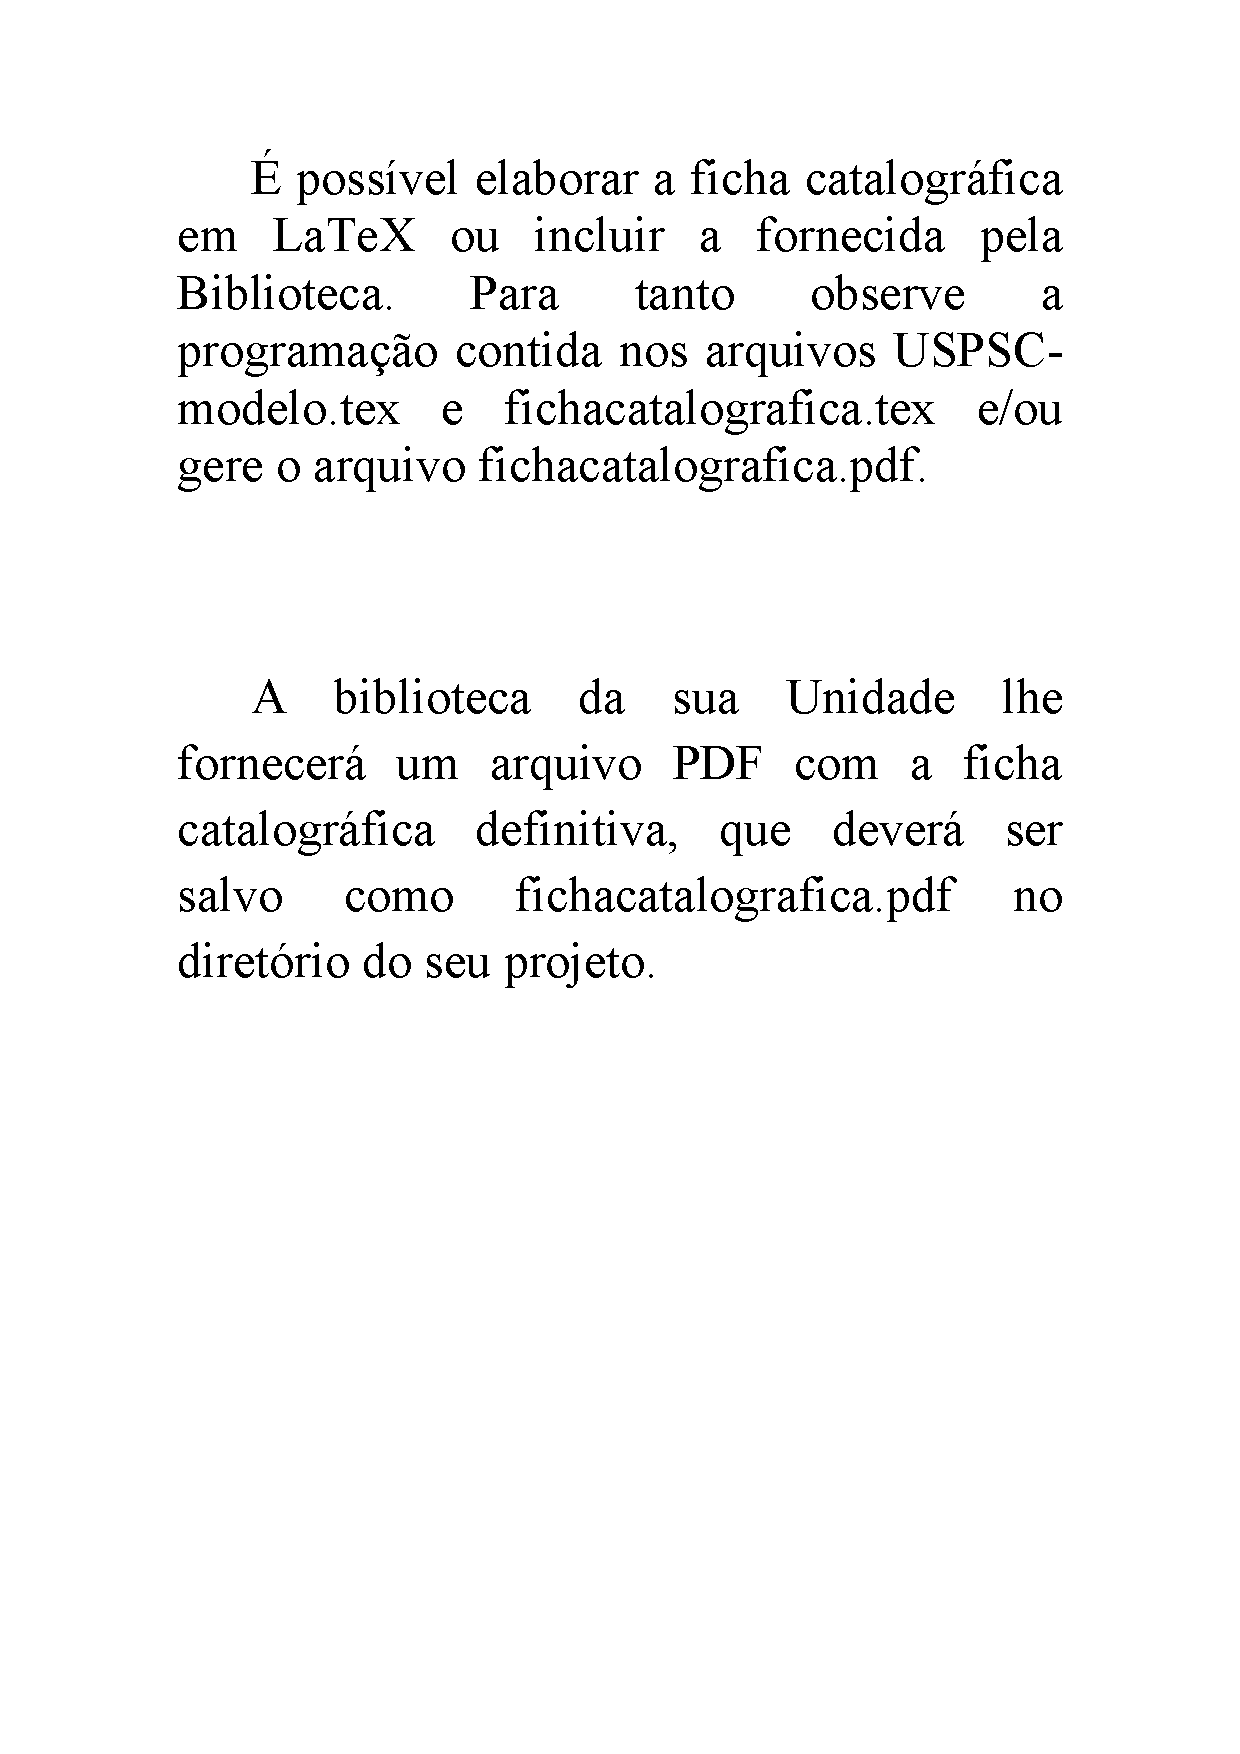
\includepdf{Model/USPSC-TA-PreTextual/USPSC-fichacatalografica.pdf}

% Se você optar por elaborar a ficha catalográfica, deverá
% incluir uma % antes da linha % antes
% do comando %% USPSC-fichacatalografica.tex
% ---
% Inserir a ficha bibliografica
% ---
% Isto é um exemplo de Ficha Catalográfica, ou ``Dados internacionais de
% catalogação-na-publicação''. Você pode utilizar este modelo como referência. 
% Porém, provavelmente a biblioteca da sua universidade lhe fornecerá um PDF
% com a ficha catalográfica definitiva após a defesa do trabalho. Quando estiver
% com o documento, salve-o como PDF no diretório do seu projeto e substitua todo
% o conteúdo de implementação deste arquivo pelo comando abaixo:
%
\begin{fichacatalografica}
	\hspace{-1.4cm}
	%\sffamily
	\vspace*{\fill}					% Posição vertical
\begin{center}					% Minipage Centralizado
  \imprimirnotabib \\
  \begin{table}[htb]
	\scriptsize
	\centering	
	\begin{tabular}{|p{0.9cm} p{8.7cm}|}
		\hline
	      & \\
		  &	  \imprimirautorficha     \\
		
		 \imprimircutter & 
							\hspace{0.4cm}\imprimirtitulo~  / ~\imprimirautor~ ;  ~\imprimirorientadorcorpoficha. -- 	\imprimirlocal, \imprimirdata.   \\
		
		  &  % Para incluir nota referente à versão corrigida no corpo da ficha,
			  % incluir % no início da linha acima e tirar a % do início da linha abaixo
			  %	\hspace{0.4cm} \imprimirtitulo~  / ~\imprimirautor~ ; ~\imprimirorientadorcorpoficha~- ~\imprimirnotafolharosto. -- \imprimirlocal, \imprimirdata.  \\
		
			\hspace{0.4cm}\pageref{LastPage} p. : il. (algumas color.) ; 30 cm.\\ 
		   % Para incluir nota referente à versão corrigida em notas,
		    % incluir uma % no início da linha acima e	
		    % tirar a % do início da linha abaixo
		    % & \hspace{0.4cm}\imprimirnotafolharosto \\ 
		  & \\ 
		  & \hspace{0.4cm}1. Machine Learning. 2. Flight Delay. 3. Graphs I. Filipe Alves Neto Verri. II. Universidade de São Paulo. III. Instituto de Ciências Matemáticas e de Computação. IV. Graph ML for Flight Delay Prediction due to Holding Manouver
		  \\
		  \hline
	\end{tabular}
  \end{table}
\end{center}
\end{fichacatalografica}
% ---


% e retirar o % do comando abaixo
%% USPSC-fichacatalografica.tex
% ---
% Inserir a ficha bibliografica
% ---
% Isto é um exemplo de Ficha Catalográfica, ou ``Dados internacionais de
% catalogação-na-publicação''. Você pode utilizar este modelo como referência. 
% Porém, provavelmente a biblioteca da sua universidade lhe fornecerá um PDF
% com a ficha catalográfica definitiva após a defesa do trabalho. Quando estiver
% com o documento, salve-o como PDF no diretório do seu projeto e substitua todo
% o conteúdo de implementação deste arquivo pelo comando abaixo:
%
\begin{fichacatalografica}
	\hspace{-1.4cm}
	%\sffamily
	\vspace*{\fill}					% Posição vertical
\begin{center}					% Minipage Centralizado
  \imprimirnotabib \\
  \begin{table}[htb]
	\scriptsize
	\centering	
	\begin{tabular}{|p{0.9cm} p{8.7cm}|}
		\hline
	      & \\
		  &	  \imprimirautorficha     \\
		
		 \imprimircutter & 
							\hspace{0.4cm}\imprimirtitulo~  / ~\imprimirautor~ ;  ~\imprimirorientadorcorpoficha. -- 	\imprimirlocal, \imprimirdata.   \\
		
		  &  % Para incluir nota referente à versão corrigida no corpo da ficha,
			  % incluir % no início da linha acima e tirar a % do início da linha abaixo
			  %	\hspace{0.4cm} \imprimirtitulo~  / ~\imprimirautor~ ; ~\imprimirorientadorcorpoficha~- ~\imprimirnotafolharosto. -- \imprimirlocal, \imprimirdata.  \\
		
			\hspace{0.4cm}\pageref{LastPage} p. : il. (algumas color.) ; 30 cm.\\ 
		   % Para incluir nota referente à versão corrigida em notas,
		    % incluir uma % no início da linha acima e	
		    % tirar a % do início da linha abaixo
		    % & \hspace{0.4cm}\imprimirnotafolharosto \\ 
		  & \\ 
		  & \hspace{0.4cm}1. Machine Learning. 2. Flight Delay. 3. Graphs I. Filipe Alves Neto Verri. II. Universidade de São Paulo. III. Instituto de Ciências Matemáticas e de Computação. IV. Graph ML for Flight Delay Prediction due to Holding Manouver
		  \\
		  \hline
	\end{tabular}
  \end{table}
\end{center}
\end{fichacatalografica}
% ---


% As informações que compõem a ficha catalográfica estão
% definidas no arquivo USPSC-pre-textual-UUUU.tex
% ---

% ---
% Folha de rosto adicional
% Para imprimir a folha de rosto adicional, exigida por algumas Unidades, a exemplo do ICMC,
% retire a % antes do comando abaixo

%\imprimirfolhaderostoadic

% ---
% ---
% Inserir errata
% ---

% commented include
%%% USPSC-Errata.tex
\begin{errata}
	%\OnehalfSpacing 			
	A errata é um elemento opcional, que consiste de uma lista de erros da obra, precedidos pelas folhas e linhas onde eles ocorrem e seguidos pelas correções correspondentes. Deve ser inserida logo após a folha de rosto e conter a referência do trabalho para facilitar sua identificação, conforme a ABNT NBR 14724 \cite{nbr14724}.
	
	Modelo de Errata:
		
	\begin{flushleft} 
			\setlength{\absparsep}{0pt} % ajusta o espaçamento da referência	
			\SingleSpacing 
			\imprimirautorabr~ ~\textbf{\imprimirtituloresumo}.	\imprimirdata. \pageref{LastPage}p. 
			%Substitua p. por f. quando utilizar oneside em \documentclass
			%\pageref{LastPage}f.
			\imprimirtipotrabalho~-~\imprimirinstituicao, \imprimirlocal, \imprimirdata. 
 	\end{flushleft}
\vspace{\onelineskip}
\OnehalfSpacing 
\center
\textbf{ERRATA}
\vspace{\onelineskip}
\OnehalfSpacing 
\begin{table}[htb]
	\center
	\footnotesize
	\begin{tabular}{p{2cm} p{2cm} p{4cm} p{4cm} }
		\hline
		\textbf{Folha} & \textbf{Linha}  & \textbf{Onde se lê}  & \textbf{Leia-se}  \\
			\hline
			1 & 10 & auto-conclavo & autoconclavo\\
		\hline
	\end{tabular}
\end{table}
\end{errata}
% ---

% ---

% ---
% Inserir folha de aprovação
% ---

% A Folha de aprovação é um elemento obrigatório da NBR 4724/2011 (seção 4.2.1.3).
% Após a defesa/aprovação do trabalho, gere o arquivo folhadeaprovacao.pdf da página assinada pela banca
% e iclua o arquivo utilizando o comando abaixo:
% commented include
%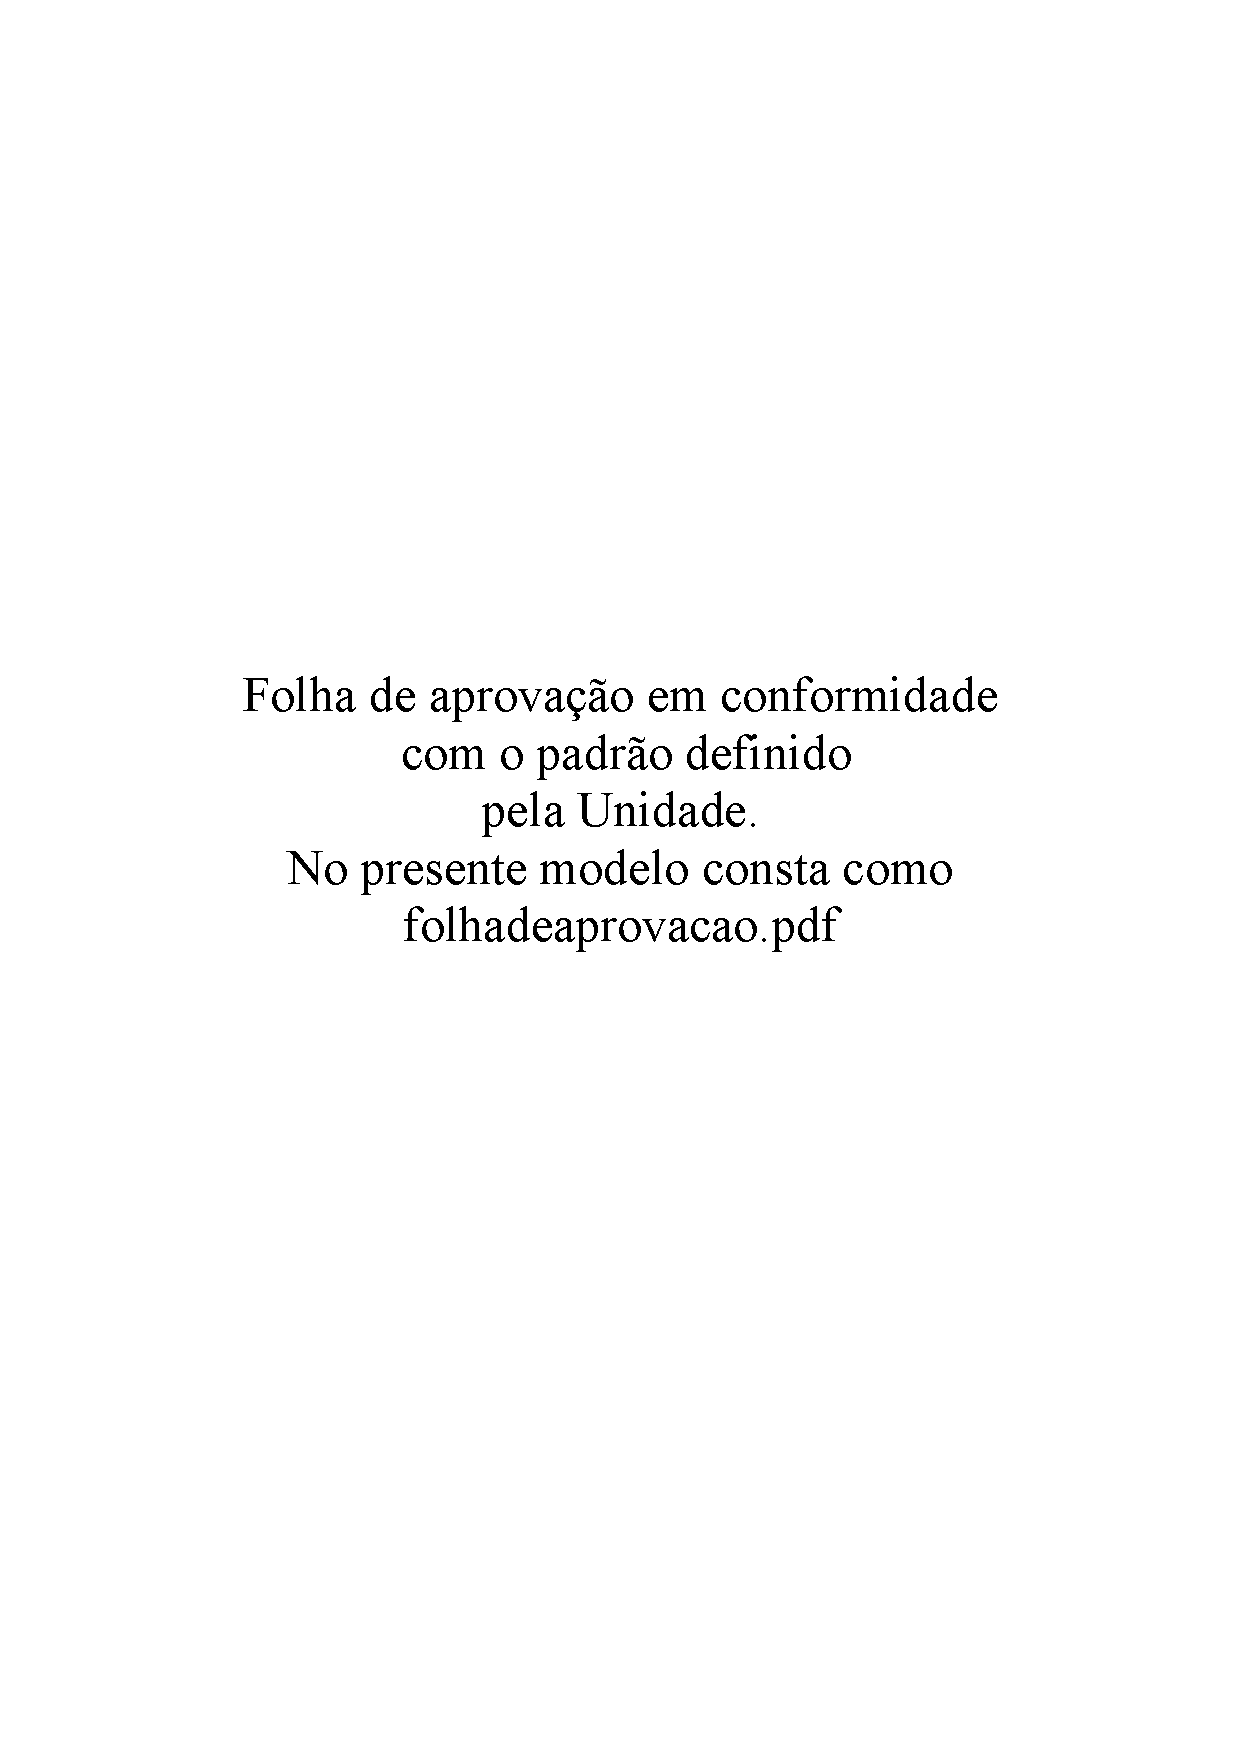
\includepdf{Model/USPSC-TA-PreTextual/USPSC-folhadeaprovacao.pdf}
% Alternativa para a Folha de Aprovação:
% Se for a sua opção elaborar uma folha de aprovação, insira uma % antes do comando acima que inclui o arquivo folhadeaprovacao.pdf,
% tire o % do comando abaixo e altere o arquivo folhadeaprovacao.tex conforme suas necessidades
%\include{folhadeaprovacao}

% commented include
%
\includepdf{Model/USPSC-TA-PreTextual/USPSC-PaginaEmBranco.pdf}

% ---
% Dedicatória
% ---
% commented include
%%% USPSC-Dedicatoria.tex
\begin{dedicatoria}
   \vspace*{\fill}
   \centering
   \noindent
   \textit{ Este trabalho é dedicado aos alunos da USP, como uma contribuição\\
  das Bibliotecas do Campus USP de São Carlos para o desenvolvimento\\
	e disseminação da pesquisa científica da Universidade.} \vspace*{\fill}
\end{dedicatoria}
% ---
% ---

% ---
% Agradecimentos
% ---
% commented include
\begin{agradecimentos}

    First and foremost, I would like to thank my family—Raul, Barbara, Sandra, and Ester—for their unwavering support throughout this journey, especially my father, João Luiz Franco, who has always encouraged my studies. It is an honor to be graduating from the same Institute and in the same course where my hero graduated in 1987. 

    I extend my deepest gratitude to my advisor, Filipe Alves Neto Verri, who has not only guided me this semester but has been a constant source of wisdom and inspiration throughout much of my academic journey. Thank you for your patience, guidance, encouragement and the opportunity you gave me, professor.

    My heartfelt thanks also go to Manoel Vilela Machado, whose collaboration and friendship were instrumental in completing this work. Our numerous discussions provided invaluable learning experiences and opportunities for growth.

    I am equally grateful to the entire ICMC staff, especially the graduation service team—for their patience with my many requests—and to the library, as well as the cleaning and general services staff, whose kindness and support made ICMC feel like a second home. I owe thanks to all the professors who contributed directly to this project through their teaching, particularly in graph theory: professors Ricardo, Diego, Francisco, Rudinei, Cynthia, Luis, and João Batista. 
    
    Furthermore, I also thank my IFSP professors Renato, André, Malu, Rodrigo, Fábio and Jorge, who encouraged me to get into college. I am sure that without their support, specially from professor Renato who passed countless days helping me in physics, I would not be here. 

    To my examination board, I am deeply thankful for this opportunity. Professor Solange, the first member of the board, lectured me Artificial Intelligence, and I could learn so much from someone that always brought a positive outlook and saw the best in us. Maria Carolina Monard, who advised both Solange and my father, was instrumental in my father's journey and consequently mine. Though she is no longer with us, I dedicate this project to her in recognition of her incredible contributions to all our lives. It is also a privilege to have my dear friend André Fakhoury as the second member of the board. Thank you for everything, André—it's interesting that this project is about graphs, but you've been helping me with graphs even before I entered at USP, back when I would bother you in GEMA's group.

    Lastly, I thank the love of my life, Isis, for making me happier every day, for all the care and understanding during this period, my friends for their unwavering support, and God, who has never abandoned me.

\end{agradecimentos}

% ---

% ---
% Epígrafe
% ---
% commented include
%% USPSC-Epigrafe.tex
\begin{epigrafe}
    \vspace*{\fill}
	\begin{flushright}
		\textit{``All people are born as originals but many die as photocopies. ''\\
		Carlo Acutis}
	\end{flushright}
\end{epigrafe}
% ---
% ---

% A T E N Ç Ã O
% Se o idioma do texto for em inglês, o abstract deve preceder o resumo
% resumo em português
%
% Resumo
% ---
% commented include
%\include{Model/USPSC-TA-PreTextualUSPSC-Resumo}
% ---

% Abstract
% ---
\begin{resumo}[Abstract]
\begin{otherlanguage*}{english}
	\begin{flushleft} 
			\setlength{\absparsep}{0pt} % ajusta o espaçamento da referência	
			\SingleSpacing 
			\imprimirautorabr~~\textbf{\imprimirtituloresumo}.	\imprimirdata. \pageref{LastPage}p. 
			%Substitua p. por f. quando utilizar oneside em \documentclass
			%\pageref{LastPage}f.
			\imprimirtipotrabalho~-~\imprimirinstituicao, \imprimirlocal, \imprimirdata. 
 	\end{flushleft}
\OnehalfSpacing
	
The growing demand for efficient last-mile delivery solutions, driven by the rise of e-commerce and urbanization, necessitates innovative approaches to manage the complexities of urban logistics. This study investigates the use of drones for last-mile delivery through a graph-based approach, focusing on the Multi-Agent Pathfinding (MAPF) problem, which involves routing multiple drones to deliver packages efficiently. Most algorithms proposed for the Last Mile Delivery Drones (LMDD) problem tend to overlook the inherent complexities of the MAPF problem. This research adopts a graph-based representation of the delivery area, transforming the problem into a network flow optimization. The proposed graph-based heuristic method is evaluated against a purely Mixed Integer Linear Programming (MILP)-based solution. Experimental results demonstrate that the heuristic approach not only enhances computational efficiency but also maintains high solution quality. Specifically, the heuristic outperforms MILP in terms of runtime while achieving comparable accuracy in path optimization. Additionally, a hybrid implementation combining heuristic and MILP is proposed. The exact MILP model has exponential complexity time as the number of drones is increased, which is expected since the MAPF paradigm is NP-Complete. The complexity of the heuristic is bounded by \(\mathcal{O}(N^3 K \max{(\log N, \log K)})\), where $K$ is the number of drones and $N$ is the dimension, if the grid is square. The study highlights the potential of centralized control systems for managing a fleet of delivery drones. The findings from extensive simulations indicate that the graph-based heuristic effectively balances computational efficiency and operational reliability, making it a viable solution for real-world last-mile delivery applications. This research contributes to the broader field of drone logistics by offering a scalable and robust method for optimizing drone delivery paths, thereby supporting the integration of drones into commercial delivery systems.  


   \vspace{\onelineskip}
 
   \noindent 
   \textbf{Keywords}: Optimization. Graphs. Last Mile Delivery Drones.
 \end{otherlanguage*}
\end{resumo}

%% USPSC-Resumo.tex
\setlength{\absparsep}{18pt} % ajusta o espaçamento dos parágrafos do resumo		
\begin{resumo}
	\begin{flushleft} 
			\setlength{\absparsep}{0pt} % ajusta o espaçamento da referência	
			\SingleSpacing 
			\imprimirautorabr~~\textbf{\imprimirtituloresumo}.	\imprimirdata. \pageref{LastPage}p. 
			%Substitua p. por f. quando utilizar oneside em \documentclass
			%\pageref{LastPage}f.
			\imprimirtipotrabalho~-~\imprimirinstituicao, \imprimirlocal, \imprimirdata. 
 	\end{flushleft}
\OnehalfSpacing 	

A crescente demanda por soluções eficientes de entrega de última milha, impulsionada pelo crescimento do comércio eletrônico e urbanização, exige abordagens inovadoras para gerenciar as complexidades da logística urbana. Este estudo investiga o uso de drones para entrega de última milha por meio de uma abordagem baseada em grafos, focando no problema de Multi-Agent Pathfinding (MAPF), que envolve o roteamento de múltiplos drones para entregar pacotes de forma eficiente. A maioria dos algoritmos propostos para o problema de Drones de Entrega de Última Milha (LMDD, em inglês) tendem a ignorar as complexidades inerentes do problema MAPF. Esta pesquisa adota uma representação baseada em grafos da área de entrega, transformando o problema em uma otimização de fluxo de rede. O método heurístico baseado em grafos proposto é avaliado em comparação com uma solução puramente baseada em Programação Linear Inteira Mista (MILP, em inglês). Os resultados experimentais demonstram que a abordagem heurística não apenas melhora a eficiência computacional, mas também mantém alta qualidade nas soluções. Especificamente, a heurística supera a MILP em termos de tempo de execução, enquanto alcança uma precisão comparável na otimização de caminhos. Além disso, é proposta uma implementação híbrida combinando heurística e MILP. O modelo MILP exato tem complexidade exponencial conforme o número de drones aumenta, o que é esperado, uma vez que o paradigma MAPF é NP-Completo. A complexidade da heurística é limitada por $\mathcal{O}(N^3 K \max{(\log N, \log K)})$, onde $K$ é o número de drones e $N$ é a dimensão, se a grade for quadrada. O estudo destaca o potencial de sistemas de controle centralizados para gerenciar uma frota de drones de entrega. Os resultados de simulações extensivas indicam que a heurística baseada em grafos equilibra a eficiência computacional e a confiabilidade operacional de forma eficaz, tornando-a uma solução viável para aplicações de entrega de última milha do mundo real. Esta pesquisa contribui para o campo mais amplo da logística de drones oferecendo um método escalável e robusto para otimizar os caminhos de entrega de drones, apoiando assim a integração de drones em sistemas de entrega comerciais. Este trabalho também sugere avanços com agentes inteligentes usando Aprendizado por Reforço (RL, em inglês) e Redes Neurais de Grafos (GNNs, em inglês) para melhorar o paradigma descentralizado, o qual nós provamos ser inferior à nossa metodologia centralizada, uma vez que utiliza uma otimização local em contraste com nossa otimização global.
 

 \textbf{Palavras-chave}: Otimização. Grafos. Drones de Entrega de Última Milha.
\end{resumo}
% ---

% ---
% inserir lista de figuras
% ---
\pdfbookmark[0]{\listfigurename}{lof}
\listoffigures*
\cleardoublepage
% ---

% ---
% inserir lista de tabelas
% ---
\pdfbookmark[0]{\listtablename}{lot}
\listoftables*
\cleardoublepage
% ---

% ---
% inserir lista de quadros
% ---
% commented include
% \pdfbookmark[0]{\listofquadroname}{loq}
% \listofquadro*
% \cleardoublepage
% ---

% ---
% inserir lista de abreviaturas e siglas
% ---
% commented include
% USPSC-AbreviaturasSiglas.tex
\begin{siglas}
    \item[\textit{GNN}] Graph Neural Network
    \item[\textit{GAT}] Graph Attention Network
    \item[\textit{ML}] Machine Learning
    \item[\textit{GCN}] Graph Convolutional Network
    \item[\textit{T-GCN}] Temporal Graph Convolutional Network
    \item[\textit{GRU}] Gated Recurrent Units
    \item[\textit{ICEA}] Instituto de Controle do Espaço Aéreo / Airspace Control Institute
    \item[\textit{SCNN}] Spectral CNN
    \item [\textit{METAR}] METeorological Aerodrome Report
    \item [\textit{METAF}] METeorological Terminal Aerodrome Forecasts
    \item [\textit{MLP}] Multilayer Perceptron
    \item [\textit{XAI}] Explainable AI 
    \item [\textit{SVM}] Support Vector Machine
    \item [\textit{SP}] São Paulo
    \item [\textit{RJ}] Rio de Janeiro
    \item[\textit{MG}] Minas Gerais 
    
\end{siglas}

% ---

% ---
% inserir lista de símbolos
% ---
% commented include
% % USPSC-Simbolos.tex
\begin{simbolos}
  \item[$ \Gamma $] Letra grega Gama
  \item[$ \Lambda $] Lambda
  \item[$ \zeta $] Letra grega minúscula zeta
  \item[$ \in $] Pertence
\end{simbolos}
% ---
% ---
% inserir o sumario
% ---
\pdfbookmark[0]{\contentsname}{toc}
\tableofcontents*
\cleardoublepage
% ---
% ----------------------------------------------------------
% ELEMENTOS TEXTUAIS
% ----------------------------------------------------------
\textual
% Os capítulos são inseridos como arquivos externos

% Capítulo 1 - Introdução
% ---
%% USPSC-Introducao.tex

% ----------------------------------------------------------
% Introdução (exemplo de capítulo sem numeração, mas presente no Sumário)
% ----------------------------------------------------------
\chapter[Introduction]{Introduction}
\label{Introdução}

Efficient last-mile delivery logistics is vital for accurate and timely delivery of goods, which influences customer satisfaction and overall business success \cite{boysen2021lastmile}. The use of drones, also called Unmanned Aerial Vehicles (UAVs), in Last-Mile Delivery improves efficiency by overcoming traffic constraints, reducing delivery times, and lowering operational costs.  For this reason, the literature on Delivery Drones increased significantly in the last few years, as analyzed in \citeonline{DUKKANCI2023}.

The literature related to Last-Mile Delivery Drones is highly heterogeneous, encompassing a diverse array of techniques and problem formulations. This diversity spans from studies involving both drones and trucks in delivery scenarios, linear integer modeling for logistic problem-solving, applications of fuzzy logic to address uncertainties, multi-objective optimization to consider multiple criteria simultaneously, to exclusive investigations focusing solely on drones without the presence of other vehicles, including decentralized models.

In \citeonline{FREITAS2023100094} it is studied the Truck-Drone Delivery Problem, which can be addressed as a variation of TSP (Traveling Salesman Problem) for two agents, using a Mixed Integer Programming (MIP) formulation and a heuristic based on a TSP solver and two metaheuristics: General Variable Neighborhood Search (GVNS) and Tabu Search (TS). At the same time, \citeonline{MOSHREFJAVADI2020290} addresses a near problem, but with multiple drones, using Mixed Integer Linear Programming (MILP) and a heuristic based on Adaptive Large Neighborhood Search (ALNS) and Simulated Annealing (SA). A similar MILP modeling was used in \citeonline{drones7070407} and two hybrid genetic algorithms were evaluated.



When addressing multiple criteria simultaneously in collaborative Truck-Drone Delivery, researchers have employed multi-objective optimization techniques.  \citeonline{9580555} consider flexible time windows and diverse objectives, including minimizing the routing costs of drones and trucks and maximizing customer satisfaction. They improved NSGA-II(Non-dominated Sorting Genetic Algorithm) and used a posterior heuristic for Pareto Local Search(PLS).   Complementing this, \citeonline{ZHANG2022108679} introduces a novel multi-objective optimization model for drone delivery, optimizing economic and environmental goals concurrently. The model addresses dynamic drone flight endurance based on loading rates, using an extended NSGA-II algorithm that proves to be effective in generating high-quality solutions, marking advancements in this field.

%Now, article fuzzy, sentiment and energy.

In another branch, works such as \citeonline{farjana2020last} introduce a systematic multi-criterion, multipersonnel decision-making approach called interval-valued inferential fuzzy TOPSIS, handling fuzziness in decision-making and providing quality drone selection decisions. Another study \citeonline{9672856} considers sustainability in optimizing the vehicle routing problem with drones, utilizing sentiment analysis based on Twitter to determine customer sentiments on environmental protection. The net promoter score index calculated from the sentiment analysis is considered as a coefficient in the penalty function added to the base model, aiming to help logistics companies improve the sustainability of the supply chain. Addressing the aspect of energy efficiency in drone-based last mile delivery, another study \citeonline{10049551} focuses on tactical decisions about the selection of shared fulfillment centers used as launch and recovery locations for drones, fleet size plans, and operational drone route decisions. 

%até aqui sem collision

A new perspective in Last Mile Delivery Drones was introduced in \citeonline{Verri}. The study addressed the last-mile delivery problem from a complex system viewpoint, where the collective performance of the drones is investigated. The delivery system incorporates a \textit{tradable permit model} \cite{AKAMATSU2017178}, based on a financial decentralized market-inspired approach, for airspace use, requiring drones to compete for airspace permits in a distributed manner. The simulation evaluates how different parameters, such as arrival rate and airspace dimensions, impact system behavior in terms of cost, time required for drones to acquire flight permits and airspace utilization. Although the simulation employs a simplified model with naïve agents and disregards drone flight dynamics, it captures interesting properties in the agents' collective behavior, demonstrating satisfactory system performance even under high traffic conditions. Simultaneously, \citeonline{lee2022last} contributes a novel combinatorial double auction bi-objective winner determination problem for last-mile drone delivery. 

As we can see, the Last Mile Delivery Drone problem is very hard and complex. In \citeonline{faical}, the authors characterize the problem through a cyber-physical lens, highlighting challenges related to the physical aspects of airspace in the context of drone operations for last-mile delivery. Their analysis delves into considerations such as air traffic management systems, focusing on the evolving landscape of airspace control. This review underscores the need for optimal usage of airspace, then ensuring the need for collision avoidance. However, collision avoidance is a problem that has not been addressed by most of the cited papers until now. \citeonline{Verri} addresses this systematically within the decentralized approach. Indeed, \citeonline{DUKKANCI2023} highlights collision avoidance and air traffic management as a crucial aspect that needs attention in Last-mile delivery drone problems, as much of the literature tends to overlook this when modeling the problem. 


With this problem of collision avoidance and efficient airspace control in mind, the main idea of our work is solve the Last Mile Delivery Drone problem using a MAPF (Multi-Agent Path Finding) approach, thus not ignoring spatial characteristics natural from the airspace. The problem addressed in this work can easily be seen as multi-objective drone path planning for search and rescue \cite{hayat2020multi}, thus the Last Mile Delivery Drone is per se a MAPF.  As stated in \citeonline{lavalle} and proved in \citeonline{Nebel_2020} the MAPF problem is NP-hard. Then our approach is to use elements of prioritized planning \cite{7138650} and conflict-based search \cite{SHARON201540} to face the computational complexity inherited from MAPF while satisfying the constraints of the reduced problem. Although our algorithm does not guarantee global optimum, it always converges in a finite and bounded polynomial time, which is an improvement compared to the previous algorithms described ( MILPs, MOEAs, Metaheuristics).



Centralized control for airspace management, particularly under the Unmanned Aircraft System Traffic Management (UTM) framework developed by the Federal Aviation Administration (FAA) and NASA, exemplifies the necessity of organized, legislative-backed airspace control \cite{nasa}. The UTM facilitates multiple drone operations beyond visual line of sight (BVLOS) by enabling cooperative interaction between drone operators and the FAA, determining and communicating real-time airspace status. While decentralized models, such as those based on blockchain technology \cite{Verri}, offer novel approaches, they introduce complexities in scalability, regulatory compliance, and operational efficiency that can hinder real-time airspace control. The centralized UTM system, supported by regulatory compliance and legislative backing, ensures effective airspace management, safety, and reliability, fostering the integration of UAV deliveries within existing air traffic systems. The FAA's UTM Implementation Plan \cite{9256745} and ongoing evaluations highlight the continual refinement of this centralized approach, emphasizing its critical role in future UAV operations. 


In this study, we propose a novel approach to tackle the Last Mile Delivery Drone problem by employing a Multi-Agent Path Finding (MAPF) strategy. Leveraging elements of prioritized planning and conflict-based search, our algorithm aims to address the computational complexity inherent in the MAPF problem. Unlike previous algorithms such as MILPs and MOEAs, our heuristic guarantees convergence in finite and bounded polynomial time, representing a significant advancement. Our graph-based approach, employing Breadth-First Search (BFS) on temporal grids, enhances the efficiency of our solution. Also, we propose a hybrid method, that combines the heuristic and the MILP. We further present experimental results, comparing our approach with a MILP-based solution and evaluating its performance in the hybrid approach that combines the time found by the heuristic and the MILP solution. Finally, a qualitative comparison between our centralized approach and the decentralized, proposed in \citeonline{Verri}, is presented. The use of a graph-based heuristic offers distinctive advantages, and our experiments shed light on its efficacy in solving the complex Last Mile Delivery Drones problem.

Therefore, in what follows, we describe the main contributions
of this work:
\begin{itemize}
    \item We develop a MILP model to solve the LMDD problem exactly. This model offers a novel method to adapt the MAPF solution to the LMDD context, allowing for drone take-offs, waiting in airspace, and correct landings.
    \item We propose a heuristic algorithm to address the LMDD problem. The primary advantage of our heuristic lies in its graph-based structure, which can be adapted to higher dimensions and weighted sets in the LMDD context. Additionally, our heuristic is polynomially bounded with a low computational cost, representing a novel contribution to the current literature on drone delivery solutions.
\end{itemize}




This monograph is organized as follows. In Section 2 we present the problem definition and the new property. The proposed solution approach is described in Section 3, while the results of the computational experiments are presented in Section 4. Finally, in Section 5 conclusions are drawn.


% ---

% ---
% Capítulo 2

\chapter[Theoretical Framework]{Theoretical Framework and Related Works}
\label{TheoreticalFramework}

Graph machine learning can be tracked backwards to the problem of `learning' on data that is inherently a graph \cite{silva2016machine, JMLR:Perozzi} or can be modeled as a graph \cite{verri2013,grape2020}. This field encompasses a variety of tasks, including node/edge classification, network construction, link prediction, graph classification, graph cut/partitioning, network embeddings, graph coarsening/reduction, which rely on learning representations from graph-structured data. Over the last decades, researchers have developed numerous approaches to tackle these challenges, initially these techniques were most developed by complex networks researchers. However, in the last decade with the advancements in deep learning, the field has seen a significant shift towards the merging of three main communities: graph signal processing, deep learning and complex nets.

As described, defining the field of graph machine learning is not straightforward, as it encompasses a broad range of methods and applications. The tasks mentioned above are just a few examples of the many challenges that can be addressed through graph-based learning techniques. For clarity, these tasks can be categorized into three main learning paradigms: supervised, unsupervised, and semi-supervised learning. In this study, we are interested on the (semi-)supervised learning paradigm, which encompasses a variety of techniques designed to leverage learning to (partially-)labeled data \cite{verri2018advantages,amanciof}. But we can refine even more, in fact, this work will focus in the subset of graph elements prediction(classification/regression) methods.

In this chapter, we provide an overview of the theoretical framework of graph machine learning for node/edge prediction. Here we consider the division of the field into \texttt{classical} graph learning and \texttt{deep} graph learning, where here `classical' refers to the machine learning techniques applied to graphs before the advent of graph neural networks, where standard ML algorithms were applied to graph data and the topological information measures were encoded as features together with the tabular data  \cite{costa2007characterization, silva2016machine}. This bipartition is what will pave the way of our explanation, since the last decade has seen a complex interplay between these two approaches. The field's evolution can be traced back to when \citeonline{bruna2013spectral} introduced one of the first GNN architectures leaned on the theory of graph signal processing. Concurrently, researchers were developing node embedding techniques like DeepWalk \cite{perozzi2014deepwalk} and node2vec \cite{grover2016node2vec}, which bridged classical and deep approaches while remaining using complex networks concepts. The subsequent years saw a surge in GNN architectures, including Graph Convolutional Networks(GCNs) \cite{kipf2016semi} and GraphSAGE \cite{hamilton2017inductive}, marking a shift towards more sophisticated deep learning approaches for graphs and the unification of the field.  

In the following sections, we explain each subset, their theory and applications, and how they have evolved over time. We also discuss the challenges and limitations of these methods.

\section{Classical graph learning}

These early efforts focused on shallow learning techniques such as feature engineering, graph traversal algorithms, and spectral methods, which laid the foundation for understanding graph structure and dynamics. Methods like community detection, centrality measures, and link prediction \cite{silva2016machine} became key tools for analyzing large-scale networks in areas such as social science, biology, and infrastructure systems \cite{newman2018networks,boccaletti2006complex}. A significant focus of these techniques was to develop graph-based features that could be integrated into traditional machine learning models, effectively transforming graph data into a format compatible with standard algorithms like logistic regression, decision trees, and support vector machines. By encoding graph topology through hand-crafted features, such as connectivity and centrality, researchers could leverage these features for tasks like classification, regression, and clustering in tabular machine learning frameworks.

Among these features, centrality measures became particularly important due to their ability to capture the relative importance or influence of nodes in a graph, not just nodes \cite{bonacich1987power}, but other graph elements such as edges \cite{Lu2013edgebetw, brohl2019centrality} and hyperedges \cite{tudisco2021hyperedge}. Centrality measures, such as degree, betweenness, and closeness, served as input features in machine learning pipelines, helping to predict outcomes based on the structural role of nodes within the network. 

Spectral centrality, particularly eigenvector centrality \cite{bonacich1987power}, has proven valuable in machine learning applications due to its ability to identify globally influential nodes. Eigenvector centrality assigns a score to each node by considering not only its direct connections but also the centrality of its neighbors, which results in a recursive definition. Mathematically, the eigenvector centrality $x$ of a node in a graph can be defined as the solution to the equation $Ax = \lambda x$, where $A$ is the adjacency matrix of the graph, and $\lambda$ is the largest eigenvalue, thus $x$ is the eigenvector associated with the largest eigenvalue. This relationship arises from the fact that the centrality of a node is proportional to the sum of the centralities of its neighbors, if we normalize the adjacency we get an stochastic matrix and then $\lambda =1 $ is the largest eigenvalue, named the \texttt{Perron vector}. The eigenvector centrality captures both local and global structure in a network, making it a powerful feature for tasks such as node classification, ranking, and recommendation systems. A related and widely used spectral measure is PageRank \cite{brin1998pagerank}, which extends the idea of eigenvector centrality by introducing a damping factor to model random surfing behavior,
\[
PR(v) = \frac{1 - d}{N} + d \sum_{u \in \mathcal{N}(v)} \frac{PR(u)}{\text{deg}(u)},
\]
where $PR(v)$ is the PageRank score of node $v$, $d$ is the damping factor, and $\mathcal{N}(v)$ represents the neighbors of node $v$. This iterative computation converges to a stationary distribution of scores, which can be interpreted as the probability of landing on a given node after a long random walk, in this sense the \texttt{Perron vector} signifies the convergence of the process in the infinite. PageRank has been widely used in ranking tasks, such as identifying important websites in search engines or recommending influential users in social networks.

However, these spectral-based centralities come with limitations. Eigenvector centrality requires the computation of the principal eigenvector of the adjacency matrix, which involves finding the largest eigenpair problem. This has a time complexity of $\mathcal{O}(n^2 d)$ for exact methods, where $n$ is the number of nodes in the graph and $d$ is the ratio of convergence for the power method. Furthermore, spectral methods can suffer from limitations rooted in the Perron-Frobenius theorem, which guarantees the existence of a unique largest eigenvalue only for irreducible, non-negative matrices. For graphs that are disconnected or have negative weights, these conditions are violated, and the eigenvector centrality may not be well-defined or interpretable. That is, the adjacency matrix should be non-negative and irreducible, where we could use the Perron test $\sum A^k > 0$ to see if the graph is strongly connected.  These centralities also tend to be node-centric, lacking a direct extension to edge importance. For edge centrality, betweenness remains crucial, particularly in directed graphs, where the structural role of links (edges) must be considered to capture flow dynamics. Additionally, spectral centralities can be sensitive to noise and small perturbations in the graph structure, leading to instability in the centrality scores. Despite these challenges, spectral centrality remains a powerful tool for machine learning tasks that benefit from capturing global graph structure, provided that the computational and stability issues can be managed.


\section{Deep graph learning}

The rise of deep learning has revolutionized the field of graph machine learning, enabling the development of more powerful and scalable models for graph data. Graph neural networks can be divide in two main categories: spectral-based and spatial-based. Here is a trick thing, the GCN architecture \cite{kipf2016semi} is commonly divulgated as a spatial-based method, since it is more intuitive talking about the convolution operation in the spatial domain, where we simply aggregate information from the immediate neighbors. However, the GCN is a spectral-based method, in fact, it can be thought as a simplification of the first spectral GNN \cite{bruna2013spectral} proposed and that builds the math behind GCNs. That said, first we introduce the spectral-based GNNs and then the spatial-based ones.

\subsection{Spectral-based GNNs}

Spectral methods are rooted in graph signal processing. The core idea is that a signal on a graph can be represented as node features, where each feature vector at a node corresponds to a `signal' defined over the graph. In this context, the graph Laplacian $\mathcal{L} = D - A$, where $D$ is the degree matrix and $A$ is the adjacency matrix, plays a crucial role. It captures the structure of the graph and can be used to perform operations analogous to Fourier transforms in classical signal processing. Spectral methods can be categorized into two types: eigenvalue-based, where the focus is on creating a graph filter in the Fourier domain, and eigenvector-based, where the goal is to use a spectral basis to decompose the signal \cite{bo2023surveyspectralgraphneural}.

\citeonline{bruna2013spectral} introduced the first spectral Graph Neural Network (GNN), termed the Spectral CNN (SCNN), which aimed to translate ideas from standard Convolutional Neural Networks for images to graphs. The SCNN leverages the spectral decomposition of the graph Laplacian $\mathcal{L} = U \Lambda U^T$ to define a filter convolution operation in the Fourier domain. In this framework, the graph Fourier transform of a signal $f$ is represented as $\hat{f} = U^T f$, and the convolution operation ($\star$) is defined as $g_{\theta} \star f = U g_{\theta} U^T f$, where $g_{\theta}$ is a learnable filter parameterized by $\theta$. While powerful, the SCNN faces significant challenges: it requires $\mathcal{O}(n^3)$ computational complexity to calculate the entire graph spectrum, which is prohibitively expensive for large graphs. Moreover, the non-localized nature of eigenvectors means global information can overshadow local structural details, leading suboptimal balance between local and global information aligned with a huge parameter complexity \cite{usgnn}.

To address these limitations, ChebNet\citeonline{defferrard2016convolutional} introduces Chebyshev polynomials to approximate spectral filters, effectively reducing computational complexity while preserving the ability to capture localized patterns in the graph structure. The main ideia is to redefine our previous filtering operation to $ g_{\theta}(\mathcal{L} ) f = \sum_{k=0}^{K-1} \theta_k T_k(\widetilde{\mathcal{L}}) f $, where $T_k(\widetilde{\mathcal{L}}) = $ is the Chebyshev polinomial of order k evaluated at the scaled Laplacian $\widetilde{\mathcal{L}} = 2 \frac{\mathcal{L}}{\lambda_\text{max}} - I_n$. This innovation not only makes spectral GNNs more scalable to larger graphs, since we just need to calculate the first eigenpair ($\mathcal{O}(n^2)$ through the power method) for the approximations, but also enhances their ability to balance local and global information processing. In fact, the filters are $K$-localized for polinomials of order $K$, that is intuitive by remembering that $\mathcal{L} ^K$ represents the paths with length less or equal to $K$.  
The ChebNet laid the foundation for GCNs \cite{kipf2016semi}. Although GCNs are commonly referred to as spatial methods, their underlying principle is rooted in the truncation of the Chebyshev expansion to $K=1$, which limits the filter to first-order neighbors. This simplification reduces computational complexity significantly while preserving effectiveness. Instead of requiring the full spectral decomposition of the Laplacian matrix, GCNs use a localized approximation of the graph convolution, expressed as: $g_{\theta} \star f \approx \theta (I_n + \widetilde{A}) f$, where $\widetilde{A} = D^{-\frac{1}{2}} A D^{-\frac{1}{2}}$ is the normalized adjacency matrix, where $A$ is the adjacency matrix, and $D$ is the degree matrix. This approximation results in an efficient propagation rule that aggregates information from a node's immediate neighbors while updating the node's features. This propagation mechanism is often confused as a spatial method because it effectively propagates information from adjacent nodes—akin to a spatial neighborhood aggregation. Although its already a simple model, results have shown that GCNs can achieve state-of-the-art performance on a variety of tasks with even more simplifications \cite{wu2019simplifying}.

However, as we can note, all these spectral methods works just in undirected graphs, since it needs the spectral decomposition


\subsection{Spatial-based GNNs}

Spatial-based GNNs differ from spectral-based approaches by directly leveraging the graph structure to perform convolutions in the spatial domain, rather than relying on the spectral decomposition of graph operators like the Laplacian. In spatial-based methods, the convolution operation is interpreted as an aggregation of node features from a node's local neighborhood, akin to how standard convolutional neural networks aggregate pixel information from nearby regions in image data. These methods operate by iteratively updating node representations by propagating information between neighboring nodes, making them intuitive and highly scalable for large-scale graphs.

The general framework for message passing in spatial-based GNNs can be described as follows. For each node $i$, at layer $t$, we aggregate the features of its neighbors $\mathcal{N}(i)$ to produce an updated node embedding: $\mathbf{m}_i^{(t+1)} = \text{AGGREGATE}^{(t)} \left( \left\{ \mathbf{h}_j^{(t)} : j \in \mathcal{N}(i) \right\} \right)$, where $\mathbf{h}_j^{(t)}$ is the feature of neighboring node $j$ at layer $t$. Then, we update the node $i$'s representation: $\mathbf{h}_i^{(t+1)} = \text{UPDATE}^{(t)} \left( \mathbf{h}_i^{(t)}, \mathbf{m}_i^{(t+1)} \right)$, where $\text{AGGREGATE}^{(t)}$ is a neighborhood aggregation function, and $\text{UPDATE}^{(t)}$ is the node update function.

The general idea behind spatial-based GNNs is that, for each node, we aggregate the features of its neighbors to produce an updated node embedding. A key example of this is the GraphSAGE architecture \cite{hamilton2017inductive}, which computes node representations by sampling and aggregating features from the node's neighbors. The GraphSAGE model employs several types of aggregation functions, including mean, LSTM-based, and pooling aggregators, which allow for flexible and inductive learning on large graphs. In particular, GraphSAGE enables the generation of embeddings for unseen nodes, making it suitable for inductive learning tasks, where the model needs to generalize to new nodes that were not present during training. Unlike spectral-based methods, which are constrained to a fixed graph size and structure due to their reliance on the graph Laplacian, spatial-based GNNs are inherently more flexible and can be applied to dynamic and evolving graphs. These models perform neighborhood aggregation locally, and therefore do not require the global knowledge of the graph structure that spectral methods need. This flexibility makes them particularly useful for large-scale graphs and for graphs where the structure may change over time, such as social networks or knowledge graphs.


Another prominent spatial-based GNN is the Graph Attention Network (GAT) \cite{velickovic2017graph}, which introduced attention mechanisms into graph learning. GAT models learn to assign different weights to the neighbors of a node, allowing the model to focus more on the most relevant neighbors during the feature aggregation process. This is achieved using a self-attention mechanism, where the importance of neighboring nodes is learned through a shared attention coefficient, $
e_{ij} = \text{LeakyReLU}(\mathbf{a}^T [\mathbf{W} \mathbf{h}_i || \mathbf{W} \mathbf{h}_j]) $, where $e_{ij}$ represents the attention coefficient between nodes $i$ and $j$, $\mathbf{W}$ is a learnable weight matrix, $\mathbf{h}_i$ and $\mathbf{h}_j$ are the feature vectors of nodes $i$ and $j$, and $||$ denotes concatenation. The attention coefficients are then normalized across all of a node's neighbors using the softmax function, $
\alpha_{ij} = \frac{\exp(e_{ij})}{\sum_{k \in \mathcal{N}(i)} \exp(e_{ik})}
$, this normalization ensures that the attention coefficients sum to 1, allowing the model to perform a weighted aggregation of the neighbors' features, $
\mathbf{h}_i' = \sigma \left( \sum_{j \in \mathcal{N}(i)} \alpha_{ij} \mathbf{W} \mathbf{h}_j \right)$,
here $\mathbf{h}_i'$ is the updated representation of node $i$, and $\sigma$ is a non-linear activation function. By learning attention coefficients, GATs can capture both the importance and the structure of the graph, making them particularly effective in tasks where the relationships between nodes are not equally important, such as in citation networks or social media graphs.

% ---

%\include{6_mathematical_model}

%\include{7_heuristic}



%\include{5_materialsAndMethods}

% ---
% Capítulo 3
% ---
\chapter[Materials and Methods]{Materials and Methods}
\label{Materials}

This chapter details the materials and methods used in our study. Specifically, we will cover the dataset, the model based on CatBoost using graph-derived features, and our approach using Graph Attention Networks (GATs) for predictive modeling. Our dataset includes a range of meteorological, geographical, and flight variables. 

Our objective is to detail and model how to predict if a given aircraft is going to delay due to holding maneuver in a supervised learning setting.

\section{Datasets}
\label{Datasets}

The study utilizes two distinct datasets, each containing 42,336 observations, with identical meteorological, geographical, and flight-related features. These datasets were constructed from a combination of METAR and METAF weather reports, airport and flight specifications sourced from ICEA. Each dataset serves a different predictive modeling purpose—binary classification and regression—and includes tailored labels to reflect these objectives

One of the primary challenges in the classification dataset is its class imbalance, which could impact model performance. Common approaches to address imbalance, such as oversampling or undersampling, have been shown to introduce limitations like overfitting and poor generalization (\cite{zhao2021graphsmote}, Graph SMOTE). For graph machine learning tasks, oversampling is generally problematic due to the risk of introducing artificial connectivity patterns, while undersampling can lead to loss of critical structural information. Therefore, we opted to explore model-based techniques without applying these rebalancing methods.

\subsection{Binary Classification Dataset}
The binary classification dataset is used to predict the likelihood of a holding maneuver occurring for a given flight. In this dataset, the label is a binary value:
\begin{itemize}
    \item \textbf{Class 0 (No Holding)}: Represents flights with no holding delays, comprising 41,616 samples.
    \item \textbf{Class 1 (Holding)}: Indicates flights with holding delays, comprising only 720 samples.
\end{itemize}
This significant imbalance between the classes adds complexity to the classification task, as the model needs to accurately predict a rare event within the data.

\subsection{Regression Dataset}
The regression dataset aims to predict the exact duration of holding delays in seconds, thus providing a continuous label for each observation:
\begin{itemize}
    \item \textbf{Holding Time (Seconds)}: For this dataset, each holding event is represented by a floating-point number indicating the holding time in seconds. This approach enables a finer-grained analysis and can potentially improve operational insights by quantifying delay duration rather than merely classifying its occurrence.
\end{itemize}


\subsection{Meteorological Features}
The dataset includes a comprehensive range of meteorological variables from both METAR and METAF reports:

\begin{itemize}
    \item \textbf{Wind Direction:} \texttt{metar\_wind\_direction}, \texttt{metaf\_wind\_direction}
    \item \textbf{Wind Speed:} \texttt{metar\_wind\_speed}, \texttt{metaf\_wind\_speed}
    \item \textbf{Wind Gusts:} \texttt{metar\_wind\_gust}, \texttt{metaf\_wind\_gust}
    \item \textbf{Visibility:} \texttt{metar\_visibility}, \texttt{metaf\_visibility}
    \item \textbf{Cloud Coverage:} \texttt{metar\_cloudcover}, \texttt{metaf\_cloudcover}
    \item \textbf{Temperature:} \texttt{metar\_temperature}, \texttt{metaf\_temperature}
    \item \textbf{Dew Point:} \texttt{metar\_dewpoint}, \texttt{metaf\_dewpoint}
    \item \textbf{Altitude:} \texttt{metar\_elevation}, \texttt{metaf\_elevation}
    \item \textbf{Sky Levels:} \texttt{metar\_skylev1}, \texttt{metar\_skylev2}, \texttt{metar\_skylev3}, \texttt{metar\_skylev4}, \texttt{metaf\_skylev1}, \texttt{metaf\_skylev2}, \texttt{metaf\_skylev3}, \texttt{metaf\_skylev4}
    \item \textbf{Altimeter Setting:} \texttt{metar\_altimeter}, \texttt{metaf\_altimeter}
    \item \textbf{Weather Symbols:} \texttt{metar\_current\_wx1\_symbol}, \texttt{metar\_current\_wx2\_symbol}, \texttt{metar\_current\_wx3\_symbol}, \texttt{metaf\_current\_wx1\_symbol}, \texttt{metaf\_current\_wx2\_symbol}, \texttt{metaf\_current\_wx3\_symbol}
\end{itemize}

\subsection{Geographical Features}
The geographical features include variables based on flight paths and airport information:

\begin{itemize}
    \item \textbf{Flight Distance:} Calculated as the geodesic distance between departure and arrival airports.
    \item \textbf{Airport Altitude:} \texttt{departure\_altitude} and \texttt{arrival\_altitude}, reflecting the elevation of the airports.
    \item \textbf{Latitude and Longitude:} \texttt{departure\_latitude}, \texttt{departure\_longitude}, \texttt{arrival\_latitude}, and \texttt{arrival\_longitude} for geolocation-based analysis.
\end{itemize}

\subsection{Flight-Specific Features}
These features capture specific characteristics related to the flight and any runway head changes:

\begin{itemize}
    \item \textbf{Previous Runway Head Change:} \texttt{prev\_troca\_cabeceira}
    \item \textbf{Runway Head Change in Previous Hour:} \texttt{troca\_cabeceira\_hora\_anterior}
    \item \textbf{Flight Hour:} \texttt{hora\_do\_voo}
\end{itemize}

\section{CatBoost with Graph Features}
\label{sec:catboost_model}

This study employs the CatBoost model, a high-performance gradient boosting library, chosen specifically for its ability to handle categorical features and class imbalance effectively, as well as for its robust handling of noisy data \cite{prokhorenkova2018catboost}. CatBoost has been widely recognized for its superior performance in structured data problems, particularly when compared to other boosting algorithms like XGBoost and LightGBM, thanks to its unique techniques such as ordered boosting and categorical feature encoding. These innovations help prevent overfitting and enhance generalization in class unbalanced problems.

Here, we describe how CatBoost is combined the graph-based features that are extracted of our modeled airports network. These features are derived from the weighted directed graph and enconded as tabular features that are used as input to the model as we describe in the following sections.


\subsection{Graph Representation of the Flight Network}

\begin{figure}[ht]
    \centering
    \begin{tikzpicture}[
        ->, % directed edges
        >=stealth, % arrow tip
        node distance=3cm, % distance between nodes
        airport/.style={circle, draw, minimum size=2cm, font=\Large}, % style for airports
        flight/.style={font=\small} % style for flights
    ]

    % Nodes (Airports)
    \node[airport] (A) {SP \\ \faPlaneDeparture}; % São Paulo with departure icon
    \node[airport] (B) [right of=A] {RJ \\ \faPlaneDeparture}; % Rio de Janeiro with departure icon
    \node[airport] (C) [below of=A] {MG \\ \faPlaneDeparture}; % Minas Gerais with departure icon

    % Edges (Flights)
    \draw[->] (A) to node[flight, above] {\tikz[baseline]{\node[rotate=0]{\faPlane};}} (B); % Flight from SP to RJ, plane icon aligned (0 degrees)
    \draw[->] (B) to node[flight, right] {\tikz[baseline]{\node[rotate=220]{\faPlane};}} (C); % Flight from RJ to MG, plane icon rotated 270 degrees
    \draw[->] (C) to node[flight, left] {\tikz[baseline]{\node[rotate=96]{\faPlane};}} (A); % Flight from MG to SP, plane icon rotated 135 degrees

    \end{tikzpicture}
    \caption{Airports and Directed Flights}
    \label{fig:flight_network_graph}
\end{figure}


To model the interactions in flight data, we represented the problem as a directed graph, depicted in Figure~\ref{fig:flight_network_graph}, where each node represents an airport, here we represent the airports as states of Brazil: SP (São Paulo), MG (Minas Gerais), RJ (Rio de Janeiro). In this network:
\begin{itemize}
    \item Nodes represent airports.
    \item Directed edges represent flights, with each edge directed from the departure airport to the destination airport.
\end{itemize}
Given the frequent occurrence of multiple flights between the same pairs of airports (i.e., multiedges), we have in fact a multigraph, however we abstract it into a weighted directed graph as shown in \ref{fig:multigraph_to_weighted_graph}. Here, each edge's weight corresponds to the total number of flights between a specific pair of airports, transforming multiple directed edges into a single weighted edge. This abstraction allows us to calculate key network metrics more easily, which we then used as features in the CatBoost model.

\begin{figure}[h]
    \centering
    \begin{tikzpicture}[
        ->, % directed edges
        >=stealth, % arrow tip style
        node distance=4cm, % distance between nodes
        airport/.style={circle, draw, minimum size=2cm, font=\Large}, % style for airports
        flight/.style={font=\small, scale=0.8} % smaller size for flights
    ]
    
    % Multigraph (Left Side)
    \node[airport] (A1) {SP \\ \faPlaneDeparture}; % São Paulo with departure icon
    \node[airport] (B1) [right of=A1] {RJ \\ \faPlaneDeparture}; % Rio de Janeiro with departure icon
    \node[airport] (C1) [below of=A1, yshift=-1cm] {MG \\ \faPlaneDeparture}; % Minas Gerais with departure icon
    
    % Multiple flights in the multigraph (non-intersecting paths)
    \draw[->] (A1) to[bend left=20] node[flight, near start] {\tikz[baseline]{\node[rotate=0, scale=0.7]{\faPlane};}} (B1); % Flight 1 from SP to RJ
    \draw[->] (A1) to[bend left=40] node[flight, near start] {\tikz[baseline]{\node[rotate=0, scale=0.7]{\faPlane};}} (B1); % Flight 2 from SP to RJ
    \draw[->] (A1) to[bend left=60] node[flight, near start] {\tikz[baseline]{\node[rotate=0, scale=0.7]{\faPlane};}} (B1); % Flight 3 from SP to RJ
    
    \draw[->] (B1) to[bend right=20] node[flight, near start] {\tikz[baseline]{\node[rotate=270, scale=0.7]{\faPlane};}} (C1); % Flight 1 from RJ to MG
    \draw[->] (B1) to[bend right=40] node[flight, near start] {\tikz[baseline]{\node[rotate=270, scale=0.7]{\faPlane};}} (C1); % Flight 2 from RJ to MG
    
    \draw[->] (C1) to[bend right=20] node[flight, near start] {\tikz[baseline]{\node[rotate=135, scale=0.7]{\faPlane};}} (A1); % Flight 1 from MG to SP
    \draw[->] (C1) to[bend right=40] node[flight, near start] {\tikz[baseline]{\node[rotate=135, scale=0.7]{\faPlane};}} (A1); % Flight 2 from MG to SP
    \draw[->] (C1) to[bend right=60] node[flight, near start] {\tikz[baseline]{\node[rotate=135, scale=0.7]{\faPlane};}} (A1); % Flight 3 from MG to SP
    
    % Transformation arrow
    \node at ($(A1)!0.5!(B1)+(3.5,-2)$) {\Huge $\Rightarrow$};
    
    % Weighted Graph (Right Side)
    \node[airport] (A2) [right=6cm of A1] {SP \\ \faPlaneDeparture}; % São Paulo airport (weighted graph)
    \node[airport] (B2) [right of=A2] {RJ \\ \faPlaneDeparture}; % Rio de Janeiro airport (weighted graph)
    \node[airport] (C2) [below of=A2, yshift=-1cm] {MG \\ \faPlaneDeparture}; % Minas Gerais airport (weighted graph)
    
    % Weighted edges (single paths)
    \draw[->] (A2) to[bend left=20] node[flight, near end, yshift=0.3cm] { $W = 3$ \;} (B2); % Weighted edge from SP to RJ
    \draw[->] (B2) to[bend right=20] node[flight, near end, xshift=0.2cm] {\; \;\;\;\;\; \; $W = 2$  } (C2); % Weighted edge from RJ to MG
    \draw[->] (C2) to[bend right=20] node[flight, near end, xshift=-0.8cm] {  $W=3$  } (A2); % Weighted edge from MG to SP
    
    \end{tikzpicture}
    \caption{Transformation of a multigraph of flights into a weighted directed graph. The multigraph (left) represents multiple flights between airports. In the weighted graph (right), edges are aggregated to show total flights as weights.}
    \label{fig:multigraph_to_weighted_graph}
\end{figure}





\subsection{Graph-based Features}
The graph-based features encode essential structural information about the flight network, capturing connectivity, centrality, and robustness. These features are crucial for understanding the influence of each airport within the network and its potential impact on flight holding patterns. 

Although we have already made this simplification of the multigraph, transforming it into a weighted directed graph, we still need to extract the features from the graph and encode them as tabular data. However, this is not straightforward, as the graph measures are not directly compatible with the model.  

The modelling will impact dramatically in the resulting graph-based features. For instance, we need to calculate edge measures, but this is not so explored as node measures, so the lack of possibilities is a challenge to be overcome.  Another challenge is the direction, that is, we have to create edge measures in a directed weighted graph, which is hard, as we detailed in section \ref{classical_learning}, because most of the complex networks measures proposed are `node centric' and for undirected graphs.

With this in mind, we can observe why the weighted graph transformation was so important, since the measures available for our setting are strongly dependent to the weight (as we will detail later), and our graph is almost totally connected, so in undirected unweighted setting they would be approximately equal, leaving no information. The following graph metrics were calculated from the weighted directed graph:

\begin{itemize}
    \item \textbf{Betweenness Centrality:} Captures the relative importance of each airport in terms of the routes it controls within the network. Higher values indicate airports that serve as critical transit points.
    \item \textbf{Flow Betweenness:} Highlights the flow dynamics of connections, showing how flights tend to route through certain airports, which may correlate with congestion.
    \item \textbf{Edge Connectivity:} Indicates the robustness of airport connections, with higher values signifying more resilient routes between airports that could better handle rerouting needs.
    \item \textbf{Degree Difference:} Measures the disparity between in-degrees and out-degrees at each node, helping to identify key hubs or spokes in the network.
    \item \textbf{Google Matrix:} Based on PageRank centrality, the Google matrix provides a probabilistic transition representation for each airport, which reflects both local and global connectivity.
\end{itemize}

As we can see, these features are not commonly used in the literature. Here is where the weighted network plays a crucial role, edge betweeness centrality \cite{newman2004finding} is constructed using shortest paths in the network, thus the weight will be crucial part of it, since without it the graph is almost fully connected, the shortest path will be almost the same for all pairs of nodes. The same happens with flow betweeness centrality \cite{freeman1991centrality}, that is a measure based on electrial circuits Kirchoff law, more specifically, instead of working with shortest paths, it use the maximum flow that pass through each edge and the weight visualized as capacity will be crucial to calculate it. 

The edge connectivity is a measure of the minimum number of edges that must be removed to disconnect the graph, and the weight will be crucial to calculate it. The degree difference we stated here as a measure of the difference between the in-degree and out-degree of a node. The Google matrix is a way we derived to keep using PageRank for edges. In fact, as we detailed in section \ref{classical_learning}, althought the PageRank centrality could be applied in our graph, since it satisfieis the Perron theorem as it is always postivie and strongly connected, it is a node measure, so we have to adapt it to edges, and the Google matrix is a way to do it. 

These features enhance the CatBoost model by embedding graph-theoretic insights into its predictive capabilities, ultimately enabling a more nuanced understanding of how network dynamics relate to flight holding patterns.




\section[Graph Attention Network]{Graph Attention Network}
\label{Graph Attention Network}

As we previously described, the GAT model in section
\ref{spatial-based} has a large range of applications, from drug
discovery to fake news detection \cite{keywordsCaravanti}. The GAT
model leverages the underlying graph structure but does not rely on
explicitly computed graph-derived features like the CatBoost model
does. Instead, it learns node representations in an end-to-end manner,
enabling the model to capture the relationships between airports and
flights directly from the data.

The modelling of a GNN for our problem is a challenging task, as we
have to adapt the model to predict edge features, since `holding' is
an edge feature in our setting. In section \ref{spectral-based} we
detailed why the spectral-based GNNs are not suitable for our setting,
as they are not able to handle edge features and direction, due to
their `node-centric' approach based on the adjacency matrix. Although
spatial-based GNNs can handle direction in their majority, they are
not able to handle edge features in general, since they need to create
a way to aggregate the edge features with the neighbors' features.

The GAT model is so used because it is highly adaptable in pratically
any graph setting. As we will show, the attention mechanism detailed
in section \ref{spatial-based} can be generalized to handle edge
features, and the model can be adapted to predict edge features. In
fact, a simple concatenation ($ || $) in the attention formula already
gives us this power ,

$$ \alpha_{ij} = \sigma(\phi_1( \mathbf{a}^T [ W h_i || W h_j || W_2 e_{ij} ])) \; \; \text{,}$$

  where $e_{ij}$ are the edge features, $h_i$ and $h_j$ are the node
  features, and $W$ and $W_2$ are the weight matrices. This formula
  allows the model to focus on the relevant neighboring nodes, making
  it ideal for relational data. In our case, the edge features are the
  tabular data features with holding being part of them, which is the
  target we want to predict. This mechanism is demonstrated in Figure
  \ref{fig:gat_layer}.


\begin{figure}[h]
    \centering
   
	
    \caption{GAT Layer with multi-head attention.}

    \label{fig:gat_layer}

   

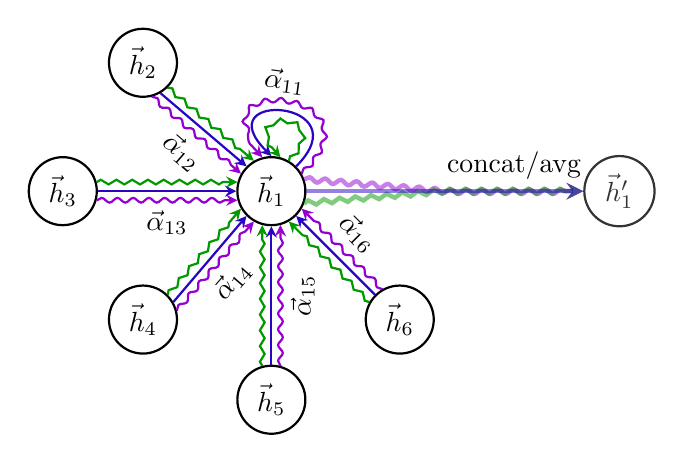
\begin{tikzpicture}

	\node[circle, draw, thick] (h1) {$\vec{h}_1$};
	\node[circle, draw, thick, above left=of h1] (h4) {$\vec{h}_2$};
	\node[circle, draw, thick, left=5em of h1] (h5) {$\vec{h}_3$};
	\node[circle, draw, thick, below left=of h1] (h6) {$\vec{h}_4$};
	\node[circle, draw, thick, below=5em of h1] (h7) {$\vec{h}_5$};
	\node[circle, draw, thick, below right=of h1] (h8) {$\vec{h}_6$};
	
	\draw[-stealth, mymauve, thick,decoration={snake, pre length=0.01mm, segment length=2mm, amplitude=0.3mm, post length=1.5mm}, decorate] (h8.120) -- node[sloped, above, black] {$\vec{\alpha}_{16}$} (h1.-30);
	\draw[-stealth, blue, thick] (h8.135) -- (h1.-45);
	\draw[-stealth, mygreen, thick, decoration={zigzag, pre length=0.01mm, segment length=2mm, amplitude=0.3mm, post length=1.5mm}, decorate] (h8.150) -- (h1.-60);
	
	\draw[-stealth, mymauve, thick,decoration={snake, pre length=0.01mm, segment length=2mm, amplitude=0.3mm, post length=1.5mm}, decorate] (h1.30) to[looseness=7] node[sloped, above, black] {$\vec{\alpha}_{11}$}(h1.105);
	\draw[-stealth, blue, thick] (h1.45) to[looseness=9] (h1.90);
	\draw[-stealth, mygreen, thick, decoration={zigzag, pre length=0.01mm, segment length=2mm, amplitude=0.3mm, post length=1.5mm}, decorate] (h1.60) to[looseness=20] (h1.75);
	
	\draw[-stealth, mymauve, thick,decoration={snake, pre length=0.01mm, segment length=2mm, amplitude=0.3mm, post length=1.5mm}, decorate] (h4.285) -- node[sloped, below, black] {$\vec{\alpha}_{12}$}(h1.150);
	\draw[-stealth, blue, thick] (h4.300) -- (h1.135);
	\draw[-stealth, mygreen, thick, decoration={zigzag, pre length=0.01mm, segment length=2mm, amplitude=0.3mm, post length=1.5mm}, decorate] (h4.315) -- (h1.120);
	
	\draw[-stealth, mymauve, thick,decoration={snake, pre length=0.01mm, segment length=2mm, amplitude=0.3mm, post length=1.5mm}, decorate] (h5.-15) -- node[sloped, below, black] {$\vec{\alpha}_{13}$}(h1.195);
	\draw[-stealth, blue, thick] (h5.0) -- (h1.180);
	\draw[-stealth, mygreen, thick, decoration={zigzag, pre length=0.01mm, segment length=2mm, amplitude=0.3mm, post length=1.5mm}, decorate] (h5.15) -- (h1.165);
	
		\draw[-stealth, mymauve, thick,decoration={snake, pre length=0.01mm, segment length=2mm, amplitude=0.3mm, post length=1.5mm}, decorate] (h6.15) -- node[sloped, below, black] {$\vec{\alpha}_{14}$}(h1.240);
	\draw[-stealth, blue, thick] (h6.30) -- (h1.225);
	\draw[-stealth, mygreen, thick, decoration={zigzag, pre length=0.01mm, segment length=2mm, amplitude=0.3mm, post length=1.5mm}, decorate] (h6.45) -- (h1.210);
	
	\draw[-stealth, mymauve, thick,decoration={snake, pre length=0.01mm, segment length=2mm, amplitude=0.3mm, post length=1.5mm}, decorate] (h7.75) -- node[sloped, below, black] {$\vec{\alpha}_{15}$}(h1.-75);
	\draw[-stealth, blue, thick] (h7.90) -- (h1.-90);
	\draw[-stealth, mygreen, thick, decoration={zigzag, pre length=0.01mm, segment length=2mm, amplitude=0.3mm, post length=1.5mm}, decorate] (h7.105) -- (h1.-105);
	
	\node[circle, draw, thick, right=10em of h1, opacity=0.8] (hp) {$\vec{h}_1'$};
	
	\coordinate[right=5em of h1] (A);
	
	\draw[-stealth,  mymauve, opacity=0.5, ultra thick,decoration={snake, pre length=0.01mm, segment length=2mm, amplitude=0.3mm, post length=1.5mm}, decorate] (h1.20) -- (A) -- (hp);
	\draw[-stealth, mygreen, opacity=0.5, ultra thick,decoration={zigzag, pre length=0.01mm, segment length=2mm, amplitude=0.3mm, post length=1.5mm}, decorate] (h1.-20) -- (A) -- (hp);
	\draw[-stealth, blue, opacity=0.5, ultra thick] (h1.0) -- (A) -- node[black, above, opacity=1.0] {concat/avg} (hp);

\end{tikzpicture}




\end{figure}

Furthermore, the directed multigraph setting we described in section
\ref{sec:catboost_model} is not a problem for the GAT model, since it
can handle multiple edges between the same pair of nodes, as we will
show in the following sections. We show how we model the GAT to be a
directed multigraph representing the flights and their features in
Figure \ref{fig:multigraph_layer}.


\begin{figure}[h]
  \centering
  \begin{tikzpicture}
    % Define colors for different attention heads
    \definecolor{color1}{RGB}{60, 120, 216}  % Blue
    \definecolor{color2}{RGB}{34, 139, 34}   % Green
    \definecolor{color3}{RGB}{255, 99, 71}   % Red

    % Define nodes
    \node[circle, draw, thick] (node1) at (0,0) {$\vec{h}_{\text{SP}}$};
    \node[circle, draw, thick] (node2) at (5,0) {$\vec{h}_{\text{RJ}}$};

    % Flight 1: alternating colors for attention heads
    \draw[-stealth, thick, color1!150] (node1) .. controls +(1,2) and +(-1,2) .. node[midway, above, black] {$\vec{\alpha}_{\text{SP},\text{RJ}}^{(\text{\faPlane}_1)}$} (node2);
    \draw[-stealth, thick, color2!150, dashed] (node1) .. controls +(1,1.5) and +(-1,1.5) .. node[midway, above, color2] {} (node2);
    \draw[-stealth, thick, color3!150, dotted] (node1) .. controls +(1,1) and +(-1,1) .. node[midway, above, color3] {} (node2);

    % Flight 2: same color pattern but lighter shades
    \draw[-stealth, thick, color1!100] (node1) .. controls +(1,-1) and +(-1,-1) .. node[midway, below, color1!70] {} (node2);
    \draw[-stealth, thick, color2!100, dashed] (node1) .. controls +(1,-1.5) and +(-1,-1.5) .. node[midway, below, black] {$\vec{\alpha}_{\text{SP},\text{RJ}}^{(\text{\faPlane}_2)}$} (node2);
    \draw[-stealth, thick, color3!100, dotted] (node1) .. controls +(1,-2) and +(-1,-2) .. node[midway, below, color3!70] { } (node2);

    % Flight 3: same color pattern but even lighter shades
    \draw[-stealth, thick, color1!50] (node1) .. controls +(1,-3) and +(-1,-3) .. node[midway, below, color1!50] { } (node2);
    \draw[-stealth, thick, color2!50, dashed] (node1) .. controls +(1,-3.5) and +(-1,-3.5) .. node[midway, below, color2!50] { } (node2);
    \draw[-stealth, thick, color3!50, dotted] (node1) .. controls +(1,-4) and +(-1,-4) .. node[midway, below, black] {$\vec{\alpha}_{\text{SP},\text{RJ}}^{(\text{\faPlane}_3)}$} (node2);

    % Output node
    \node[circle, draw, thick, right=7em of node2, opacity=0.8] (output) {$\vec{h}_{\text{RJ}}'$};

    % Aggregation line with label
    % \draw[-stealth, thick, color1!70] (node2) -- ++(1.5,0) -- ++(1.5,0) node[midway, above, black] {concat/avg} -- (output);

    \draw[-stealth,  color1, opacity=0.5, ultra thick,decoration={snake, pre length=0.01mm, segment length=2mm, amplitude=0.3mm, post length=1.5mm}, decorate] (node2.20)  -- (output);
    \draw[-stealth, color3, opacity=0.5, ultra thick,decoration={zigzag, pre length=0.01mm, segment length=2mm, amplitude=0.3mm, post length=1.5mm}, decorate] (node2.-20)  -- (output);
    \draw[-stealth, color2, opacity=0.5, ultra thick] (node2.0)  -- node[black, above, opacity=1.0] {concat/avg} (output);

  \end{tikzpicture}
  \caption{Airport multigraph GAT Layer with multi-head attention for three different flights between nodes (SP,RJ), with alternating colors opacity for each flight.}
  \label{fig:multigraph_layer}
\end{figure}


Finally, the last layer of our predictor would be to pass the learned
node embeddings $h_i$ and $h_j$ with the edge feature $e_{ij}^{(k)}$
of the flight $k$ to a fully connected layer (MLP) to predict the
holding of the flight $k$.  That is, we simply concatenate them, and
after the MLP layer, we have a sigmoid $\sigma$ activation function that
outputs the prediction $\hat{y}_k$ of holding,

$$ \hat{y}_k = \sigma (\text{MLP}(h_i || h_j || e_{ij}^{(k)})) \; \; \; \text{.} $$


\chapter{Results}
\label{Results}

% In this chapter, we describe the experiments conducted, beginning with the experimental setup and technology settings used (Section \ref{sec:setup}). We then compare the heuristic with the exact model using a fixed $T$ (obtained by the heuristic) (Section \ref{sec:comparison}), and finally, we present the phase transition in the heuristic, normalizing by individual drone paths (Section \ref{sec:transition}). This approach allows us to illustrate the advantages and limitations of our method.

% All experiments were performed on a 64-bit operating system with an Intel(R) Core(TM) i7-7700 CPU @ 3.60GHz and 16GB of RAM.

% \section{Experimental Setup and Technologies}
% \label{sec:setup}

% All experiments were conducted using the following software and tools:

% \subsection{Heuristic Implementation in C\texttt{++}}

% The heuristic approach was implemented in C\texttt{++}, chosen for its efficiency and control over system resources. Key components include:

% \begin{itemize}
% \item \textbf{Standard Library Containers}: The heuristic utilized standard C\texttt{++} library containers such as \texttt{vector} and \texttt{map} for efficient data management and manipulation. 
% \item \textbf{Version and Compiler}: The implementation made use of C\texttt{++}20, and the code was compiled using the GNU GCC compiler.
% \end{itemize}

% \subsection{Exact Model Implementation in Julia}

% The exact model was implemented in Julia, chosen for its high-performance capabilities and ease of use in mathematical and scientific computing. Key aspects include:

% \begin{itemize}
% \item \textbf{JuMP Package}: The exact model's optimization tasks were carried out using the \texttt{JuMP} package \cite{JuMPLubin2023}, a domain-specific modeling language for mathematical optimization embedded in Julia.
% \item \textbf{Gurobi Solver}: Gurobi was used as the Mixed-Integer Linear Programming (MILP) solver, interfaced through Julia, to solve the optimization problems with high precision and performance.
% \end{itemize}

% \subsection{Experimentation and Analysis}

% The comparison, experiments, and plots were conducted in Julia. The workflow included the following steps:

% \begin{itemize}
% \item \textbf{Calling C\texttt{++} Heuristic}: The compiled C\texttt{++} heuristic code was called externally from Julia. Input data was passed as files to the C\texttt{++} program.
% \item \textbf{Data Handling}: The output from the C\texttt{++} heuristic was read back into Julia for further analysis.
% \item \textbf{Visualization}: Results were plotted using the \texttt{Plots.jl} package in Julia.
% \end{itemize}

% \subsection{Drone Generation}

% The experimental setup involved generating random samples for the drones' initial and final positions, varying the number of drones and the size of the grid. For each drone $k \in \{1, \ldots, K\}$, where $K$ is the current number of drones, the starting position $(x_k^{\text{start}}, y_k^{\text{start}})$ and ending position $(x_k^{\text{end}}, y_k^{\text{end}})$ were randomly selected within a grid of size $N \times M$, where $N$ and $M$ are the dimensions of the grid.

% Formally, for each number of drones $K \in \{1, \ldots, R\}$, where $R$ is the maximum number of drones, and for each sample/trial $s \in \{1, \ldots, S\}$, the following procedure was applied:

% \begin{itemize}
% \item \textbf{Drone Generation}: For each drone $k \in \{1, \ldots, K\}$:
%   \begin{itemize}
%   \item Randomly generate $(x_k^{\text{start}}, y_k^{\text{start}}) \in \{1, \ldots, N\} \times \{1, \ldots, M\}$
%   \item Randomly generate $(x_k^{\text{end}}, y_k^{\text{end}}) \in \{1, \ldots, N\} \times \{1, \ldots, M\}$, ensuring $(x_k^{\text{end}}, y_k^{\text{end}}) \neq (x_k^{\text{start}}, y_k^{\text{start}})$
%   \end{itemize}
% \end{itemize}

% \section{Models Comparison}
% \label{sec:comparison}

% In this section, we compare the two models in terms of optimality(objective performance) and computational efficiency(running time). The x-axis in each plot represents the number of drones used to generate 20 samples per number of drones in the box plots, conducted in a 5x5 grid. The input $T$ for the exact model in each sample is the one returned by the heuristic, that is, $ T_{\text{exact\_model}} \vcentcolon  = T_{\text{heuristic}}$.

% \subsection{Objective Function Performance}

% We first evaluate the performance of both models in terms of their objective function outcomes. The objective function (y-axis) represents the optimization goal of minimizing path lengths for drones while avoiding collisions. Figure \ref{fig:exact_model_obj} and Figure \ref{fig:heuristic_obj} depict box plots comparing the objective function values achieved by the exact model and the heuristic model, respectively. 

% Figure \ref{fig:exact_model_obj} presents the distribution of objective function values obtained by the exact model, illustrating the spread and central tendency of the outcomes across different scenarios. Conversely, Figure \ref{fig:heuristic_obj} showcases the corresponding results for the heuristic model. By comparing these plots, we can gain valuable insights into the performance of each model in optimizing the objective function.

% In the scenario where $n_{\text{drones}} = 1$, the heuristic model performs as optimally as the exact model since the BFS guarantees optimality in this simple case. However, as the number of drones increases, the performance of the heuristic model diminishes. This decline in performance is anticipated due to the increased traffic within a fixed grid size, leading to more complex interactions and potential conflicts between the drones.


% \begin{figure}[H]
%     \centering
%     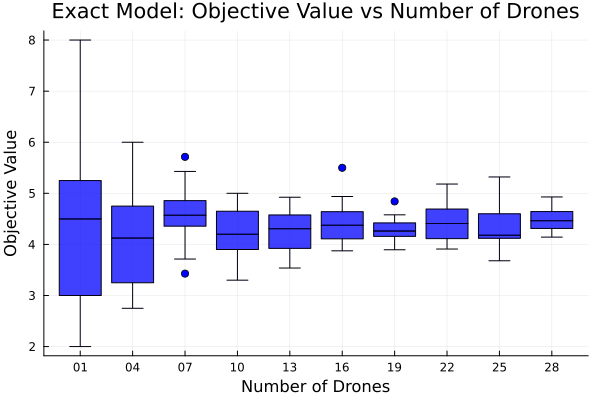
\includegraphics[width=0.8\textwidth]{img/julia_obj_boxplot_vs_drones.png}
%     \caption{Exact Model Objective. Source: The authors.}
%     \label{fig:exact_model_obj}
% \end{figure}

% \begin{figure}[H]
%     \centering
%     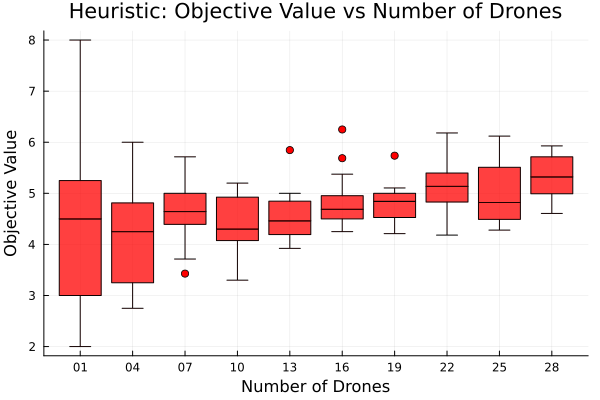
\includegraphics[width=0.8\textwidth]{img/cpp_obj_boxplot_vs_drones.png}
%     \caption{Heuristic Objective. Source: The authors.}
%     \label{fig:heuristic_obj}
% \end{figure}


% \subsection{Computational Efficiency}

% Next, we analyze the computational efficiency of the two models, focusing on the time required (y-axis) to compute the optimal paths for drones. Figures \ref{fig:exact_model_time} and \ref{fig:heuristic_time} display box plots representing the computational time taken by the exact model and the heuristic model, respectively. 

% Figure \ref{fig:exact_model_time} illustrates the distribution of computational times for the exact model. This plot provides an understanding of the computational overhead associated with solving the optimization problem precisely. Conversely, Figure \ref{fig:heuristic_time} presents the computational times required by the heuristic model. By comparing these plots, we assess the trade-off between computational efficiency and solution optimality offered by each model.

% As illustrated in Figure \ref{fig:exact_model_time}, the heuristic consistently exhibits a lower running time compared to the exact model. This disparity in running times is not merely a constant difference but reflects the inherent differences in computational complexity between the two approaches. The heuristic model demonstrates an almost constant running time, attributed to its sub-linear performance relative to the number of drones, as discussed in Section \ref{secc:complexity_analysis}. In contrast, the exact model, being NP-complete, has constraints that cause its performance to depend exponentially on both the number of drones and the specified $T$. Consequently, the running time of the exact model increases exponentially with the number of drones, as evidenced by the plot in Figure \ref{fig:exact_model_time}.


% \begin{figure}[H]
%     \centering
%     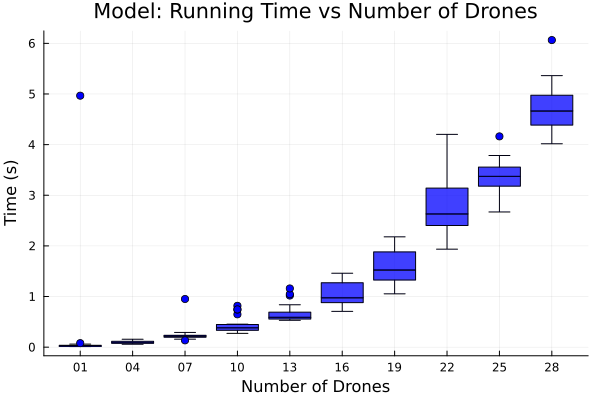
\includegraphics[width=0.8\textwidth]{img/julia_time_boxplot_vs_drones.png}
%     \caption{Exact Model time. Source: The authors.}
%     \label{fig:exact_model_time}
% \end{figure}

% \begin{figure}[H]
%     \centering
%     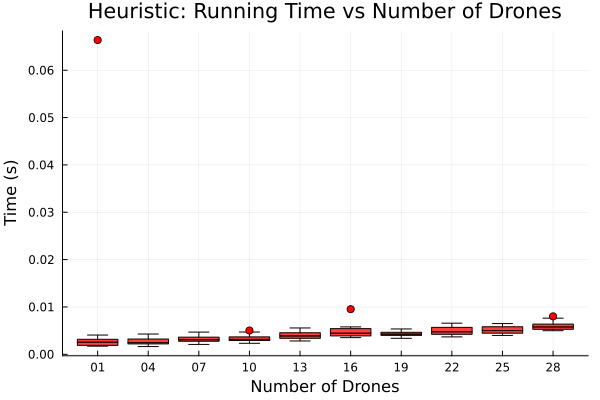
\includegraphics[width=0.8\textwidth]{img/cpp_time_boxplot_vs_drones.png}
%     \caption{Heuristic time. Source: The authors.}
%     \label{fig:heuristic_time}
% \end{figure}

% \subsection{Heuristic Behavior and Transition}
% \label{sec:transition}

% In this section, we propose an experimental setup to analyze the behavior of the heuristic in high-traffic configurations. We compare the heuristic's performance with the optimal distance for each drone in a collision-free environment, where the optimal path for each drone does not consider other drones in the grid (Manhattan distance).

% Primarily, we define the optimal distance per drone as the Manhattan distance between its start and end points. For each drone $k \in \mathcal{R}$, with starting position $(x_k^{\text{start}}, y_k^{\text{start}})$ and ending position $(x_k^{\text{end}}, y_k^{\text{end}})$, the Manhattan distance $D_k$ is given by: \[
% D_k = |x_k^{\text{start}} - x_k^{\text{end}}| + |y_k^{\text{start}} - y_k^{\text{end}}|\text{.}
% \]

% We then calculate the actual path length $P_k$ for each drone $k$ based on the heuristic path, and compute the optimality ratio $R_k$ as follows: \[
% R_k = \frac{P_k}{D_k}\text{.}
% \]

% The optimality ratio provides a measure of how efficiently the heuristic performs compared to the ideal (collision-free) path.

% The experiments were conducted using a $6 \times 6$ grid with the number of drones ranging from 1 to 99. For each number of drones, 30 points were sampled.

% The visualization of the heuristic performance can be measured in several ways. For our purpose, we chose two metrics:

% \begin{itemize}
%     \item \textbf{Normalized Distance}: This metric shows the actual path length taken by each drone normalized by the Manhattan distance. It illustrates how the heuristic manages to find paths in high-traffic scenarios compared to the optimal path lengths.
% \end{itemize}

% \begin{figure}[H]
%     \centering
%     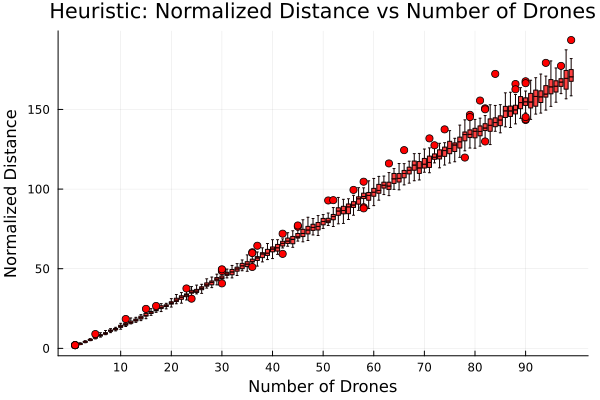
\includegraphics[width=0.8\textwidth]{img/cpp_normalized_distance_boxplot_vs_drones.png}
%     \caption{Heuristic normalized distance per drone. Source: The authors.}
%     \label{fig:heuristic_normalized_dist}
% \end{figure}

% Figure \ref{fig:heuristic_normalized_dist} displays the distribution of normalized distances for the heuristic, highlighting how the path lengths vary with an increasing number of drones. The box plot provides insights into the spread and central tendency of the heuristic's performance.

% \begin{itemize}
%     \item \textbf{Routing Time ($T$)}: This metric shows the time taken for the heuristic to compute the paths for all drones. It provides an understanding of the computational efficiency of the heuristic as the traffic increases.
% \end{itemize}

% \begin{figure}[H]
%     \centering
%     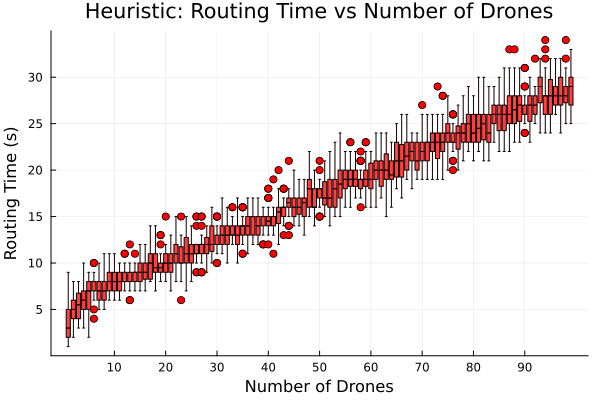
\includegraphics[width=0.8\textwidth]{img/cpp_routing_time_boxplot_vs_drones.png}
%     \caption{Heuristic Routing Time ($T$) corresponding to Figure \ref{fig:heuristic_normalized_dist}. Source: The authors.}
%     \label{fig:heuristic_normalized_routing_time}
% \end{figure}

% Figure \ref{fig:heuristic_normalized_routing_time} illustrates the routing times required by the heuristic as the number of drones increases. The box plot shows the variability in routing times and helps identify any trends or outliers. This result evinces the reasonability of the hybrid method in \ref{Hybrid_Methodology}, since we have a T that increases just linearly in the number of drones, even in a high traffic condition(36 cells available cells and 99 drones).

% Together, these figures provide a comprehensive view of the heuristic's behavior under varying traffic conditions, demonstrating both its effectiveness in finding feasible paths and its computational efficiency. 
% ---

% Capítulo 4 - Conclusão
% ---
% ---
% Conclusão
% ---
\chapter{Conclusion}
\label{Conclusion}

\section{Project Contributions to the Student}

This project was an excellent way to reinforce the knowledge I gained in my undergraduate program, particularly in areas like algorithms and graph applications. Working at ICMC was an invaluable opportunity to engage with experts in graph machine learning and complex networks. Through this project, I gained insight into both fields—a feat that would have been challenging without the foundation provided by courses like Complex Networks and Artificial Intelligence, which taught me the basics of each. Additionally, this experience provided an ideal introduction to studying \emph{graph neural networks}, a field I plan to pursue further.

\section{Relationship between the Undergraduate Course and the Project}

The undergraduate curriculum strongly aligned with this project. Key subjects included Algorithms and Data Structures, Computational Modeling in Graphs, Artificial Intelligence, High-Performance Computing, Linear Algebra, Calculus, Stochastic Processes, Statistics, and Advanced Algorithms and Applications. Together, these courses provided a comprehensive foundation in computer science, with ample focus on graph theory, machine learning, and algorithm design. The curriculum thus offered a robust theoretical framework that enriched my understanding of complex networks and graph-based models.

Another crucial aspect of my program was the opportunity to participate in teaching and research. This experience not only deepened my technical knowledge but also honed my communication skills, enabling me to articulate ideas and solutions more effectively.

\section{Reflections on the Undergraduate Course}

The Bachelor of Computer Science at the Instituto de Ciências Matemáticas e de Computação, Universidade de São Paulo, has been instrumental in providing me with knowledge, friendships, determination, and joy. I am deeply grateful for the supportive structure at ICMC, which offered everything necessary for personal and academic growth. Being surrounded by dedicated and inquisitive peers and professors has been the highlight of my time here, creating a stimulating environment that constantly pushed me to expand my horizons as a person, a scholar, and a future professional.

That said, I do have one critique regarding the course curriculum. Recently, it feels as though the Bachelor of Computer Science program has shifted its focus more toward the job market than foundational science. While I understand the need to prepare students for industry, I believe that we must preserve the course's scientific roots. For instance, `Research Methodology' is not a required course, yet it is fundamental for academic development, while other subjects more geared toward job readiness are mandatory. The removal of `Calculus 4` from the curriculum further illustrates this shift away from theoretical depth, despite its relevance in areas like machine learning.

To address this, I would suggest offering two distinct tracks within the program: an Academic Track and a Professional Track. This structure would allow students interested in research and theoretical science to focus on these areas, while those aiming for immediate industry applications could focus on practical skills. This change might also encourage more students to pursue advanced degrees at ICMC by fostering a stronger scientific foundation during their undergraduate studies.

Despite these critiques, I am confident that choosing this program was one of the best decisions I have made. The course has opened doors to opportunities I had not even dreamed of achieving.

% ---

% ---
% Capítulo de Referencia
% ---
%%% USPSC-Cap2-Desenvolvimento.tex 

% ---
% Este capítulo, utilizado por diferentes exemplos do abnTeX2, ilustra o uso de
% comandos do abnTeX2 e de LaTeX.
% ---

\chapter{Desenvolvimento}\label{cap_exemplos}
Este capítulo é parte principal do trabalho acadêmico e deve conter a exposição ordenada e detalhada do assunto. Divide-se em seções e subseções, em conformidade com a abordagem do tema e do método, abrangendo: revisão bibliográfica, materiais e métodos, técnicas utilizadas, resultados obtidos e discussão.

Abaixo são apresentados minimamente exemplos tabelas, quadros, divisões de documentos e outros itens. Consulte o \textbf{Tutorial do Pacote USPSC para modelos de trabalhos de acad\^emicos em LaTeX - vers\~ao 3.1} para demais informações. 

\section{Resultados de comandos}\label{sec-divisoes}

% ---
\subsection{Tabelas e quadros}

O \textbf{Tutorial do Pacote USPSC para modelos de trabalhos de acad\^emicos em LaTeX - vers\~ao 3.1} apresenta orientações completas e diversas formatações de tabelas, dentre elas a \autoref{tab-ibge}, que é um exemplo de tabela alinhada que pode ser longa ou curta, conforme padrão do Instituto Brasileiro de Geografia e Estatística (IBGE).

%\begin{table}[H]
\begin{table}[htb]
	\IBGEtab{%
		\caption{Frequência anual por categoria de usuários}%
		\label{tab-ibge}
	}{%
		\begin{tabular}{ccc}
			\toprule
			Categoria de Usuários & Frequência de Usuários \\
			\midrule \midrule
			Graduação & 72\% \\
			\midrule 
			Pós-Graduação & 15\% \\
			\midrule 
			Docente & 10\% \\
			\midrule 
			Outras & 3\% \\
			\bottomrule
		\end{tabular}%
	}{%
		\fonte{Elaborada pelos autores.}%
		\nota{Exemplo de uma nota.}%
		\nota[Anotações]{Uma anotação adicional, que pode ser seguida de várias
			outras.}%
		
	}
\end{table}


A formatação do quadro é similar à tabela, mas deve ter suas laterais fechadas e conter as linhas horizontais.
\newpage

% o comando \newpage foi utilizado para forçar a quebra de página

\begin{quadro}[htb]
	\caption{\label{quadro_modelo}Níveis de investigação}
	\begin{tabular}{|p{2.6cm}|p{6.0cm}|p{2.25cm}|p{3.40cm}|}
		\hline
		\textbf{Nível de Investigação} & \textbf{Insumos}  & \textbf{Sistemas de Investigação}  & \textbf{Produtos}  \\
		\hline
		Meta-nível & Filosofia\index{filosofia} da Ciência  & Epistemologia &
		Paradigma  \\
		\hline
		Nível do objeto & Paradigmas do metanível e evidências do nível inferior &
		Ciência  & Teorias e modelos \\
		\hline
		Nível inferior & Modelos e métodos do nível do objeto e problemas do nível inferior & Prática & Solução de problemas  \\
		\hline
	\end{tabular}
	\begin{flushleft}
		%\fonte{\citeonline{van1986}}
		Fonte: \citeonline{van1986}
	\end{flushleft}
\end{quadro} 


No \textbf{Tutorial do Pacote USPSC para modelos de trabalhos de acad\^emicos em LaTeX - vers\~ao 3.1} são apresentados mais exemplos de quadros.

% ---
\subsection{Figuras}\label{sec_figuras}
% ---
\index{figuras}Figuras podem ser criadas diretamente em \LaTeX,
como o exemplo da \autoref{fig_circulo}. \\ 

\begin{figure}[htb]
	\caption{\label{fig_circulo}A delimitação do espaço}
	\begin{center}
		\setlength{\unitlength}{9cm}
		\begin{picture}(1,1)
		\put(0,0){\line(0,1){1}}
		\put(0,0){\line(1,0){1}}
		\put(0,0){\line(1,1){1}}
		\put(0,0){\line(1,2){.5}}
		\put(0,0){\line(1,3){.3333}}
		\put(0,0){\line(1,4){.25}}
		\put(0,0){\line(1,5){.2}}
		\put(0,0){\line(1,6){.1667}}
		\put(0,0){\line(2,1){1}}
		\put(0,0){\line(2,3){.6667}}
		\put(0,0){\line(2,5){.4}}
		\put(0,0){\line(3,1){1}}
		\put(0,0){\line(3,2){1}}
		\put(0,0){\line(3,4){.75}}
		\put(0,0){\line(3,5){.6}}
		\put(0,0){\line(4,1){1}}
		\put(0,0){\line(4,3){1}}
		\put(0,0){\line(4,5){.8}}
		\put(0,0){\line(5,1){1}}
		\put(0,0){\line(5,2){1}}
		\put(0,0){\line(5,3){1}}
		\put(0,0){\line(5,4){1}}
		\put(0,0){\line(5,6){.8333}}
		\put(0,0){\line(6,1){1}}
		\put(0,0){\line(6,5){1}}
		\end{picture}
	\end{center}
	\legend{Fonte: \citeonline{equipeabntex2}}
\end{figure}

Consulte o \textbf{Tutorial do Pacote USPSC para modelos de trabalhos de acad\^emicos em LaTeX - vers\~ao 3.1} para conhecer mais recursos referentes à figuras. 

% ---
\section{Divisões do documento}\label{sec-divisoes-b}
Esta seção exemplifica o uso de divisões de documentos em conformidade com a ABNT NBR 6024  \cite{nbr6024}.
% ---
% ---
\subsection{Divisões do documento: subseção}\label{sec-divisoes-subsection}
% ---

Um exemplo de seção é a \autoref{sec-divisoes-b}. Esta é a \autoref{sec-divisoes-subsection}.

\subsubsection{Divisões do documento: subsubseção}\label{sec-divisoes-subsubsection}

Isto é uma \texttt{subsubsection} do \LaTeX, mas é denominada de ``subseção'' porque no português não temos a palavra ``subsubseção''.

\subsubsection{Divisões do documento: subsubseção}

Isto é outra subsubseção.

\subsection{Divisões do documento: subseção}\label{sec-exemplo-subsec}

Isto é uma subseção.

\subsubsection{Divisões do documento: subsubseção}

Isto é mais uma subsubseção da \autoref{sec-exemplo-subsec}.


\subsubsubsection{Esta é uma subseção de quinto
nível}\label{sec-exemplo-subsubsubsection}

Esta é uma seção de quinto nível. Ela é produzida com o seguinte comando:

\begin{verbatim}
\subsubsubsection{Esta é uma subseção de quinto
nível}\label{sec-exemplo-subsubsubsection}
\end{verbatim}

\subsubsubsection{Esta é outra subseção de quinto nível}\label{sec-exemplo-subsubsubsection-outro}

Esta é outra seção de quinto nível.


\paragraph{Este é um parágrafo numerado}\label{sec-exemplo-paragrafo}

Este é um exemplo de parágrafo nomeado. Ele é produzido com o comando de
parágrafo:

\begin{verbatim}
\paragraph{Este é um parágrafo nomeado}\label{sec-exemplo-paragrafo}
\end{verbatim}

A numeração entre parágrafos numerados e subsubsubseções são contínuas.

\paragraph{Esta é outro parágrafo numerado}\label{sec-exemplo-paragrafo-outro}

Este é outro parágrafo nomeado.

% ---
\subsection{Este é um exemplo de nome de subseção longa que se aplica a seções e demais divisões do documento. Ele deve estar alinhado à esquerda e a segunda e demais linhas devem iniciar logo abaixo da primeira palavra da primeira linha} 

Observe que o alinhamento do título obedece esta regra também no sumário.
	









% ----------------------------------------------------------
% ELEMENTOS PÓS-TEXTUAIS
% ----------------------------------------------------------

\postextual
% ----------------------------------------------------------

% -----------------------------------------------------------
% Referências bibliográficas
% ----------------------------------------------------------
\bibliography{8_references}


% ----------------------------------------------------------
% Glossário
% ----------------------------------------------------------
%
% Consulte o manual da classe abntex2 para orientações sobre o glossário.
%
%\glossary

% ----------------------------------------------------------
% Apêndices
% ----------------------------------------------------------
% commented include
%%% USPSC-Apendice.tex
% ---
% Inicia os apêndices
% ---

\begin{apendicesenv}
% Imprime uma página indicando o início dos apêndices
\partapendices
\chapter{Apêndice(s)}
Elemento opcional, que consiste em texto ou documento elaborado pelo autor, a fim de complementar sua argumentação, conforme a ABNT NBR 14724 \cite{nbr14724}.

Os apêndices devem ser identificados por letras maiúsculas consecutivas, seguidas de hífen e pelos respectivos títulos. Excepcionalmente, utilizam-se letras maiúsculas dobradas na identificação dos apêndices, quando esgotadas as 26 letras do alfabeto. A paginação deve ser contínua, dando seguimento ao texto principal. \cite{aguia2020}
% ----------------------------------------------------------
\chapter{Exemplo de tabela centralizada verticalmente e horizontalmente}
\index{tabelas}A \autoref{tab-centralizada} exemplifica como proceder para obter uma tabela centralizada verticalmente e horizontalmente.
% utilize \usepackage{array} no PREAMBULO (ver em USPSC-modelo.tex) obter uma tabela centralizada verticalmente e horizontalmente
\begin{table}[htb]
\ABNTEXfontereduzida
\caption[Exemplo de tabela centralizada verticalmente e horizontalmente]{Exemplo de tabela centralizada verticalmente e horizontalmente}
\label{tab-centralizada}

\begin{tabular}{ >{\centering\arraybackslash}m{6cm}  >{\centering\arraybackslash}m{6cm} }
\hline
 \centering \textbf{Coluna A} & \textbf{Coluna B}\\
\hline
  Coluna A, Linha 1 & Este é um texto bem maior para exemplificar como é centralizado verticalmente e horizontalmente na tabela. Segundo parágrafo para verificar como fica na tabela\\
  Quando o texto da coluna A, linha 2 é bem maior do que o das demais colunas  & Coluna B, linha 2\\
\hline
\end{tabular}
\begin{flushleft}
		Fonte: Elaborada pelos autores.\
\end{flushleft}
\end{table}

% ----------------------------------------------------------
\chapter{Exemplo de tabela com grade}
\index{tabelas}A \autoref{tab-grade} exemplifica a inclusão de traços estruturadores de conteúdo para melhor compreensão do conteúdo da tabela, em conformidade com as normas de apresentação tabular do IBGE.
% utilize \usepackage{array} no PREAMBULO (ver em USPSC-modelo.tex) obter uma tabela centralizada verticalmente e horizontalmente
\begin{table}[htb]
\ABNTEXfontereduzida
\caption[Exemplo de tabelas com grade]{Exemplo de tabelas com grade}
\label{tab-grade}
\begin{tabular}{ >{\centering\arraybackslash}m{8cm} | >{\centering\arraybackslash}m{6cm} }
\hline
 \centering \textbf{Coluna A} & \textbf{Coluna B}\\
\hline
  A1 & B1\\
\hline
  A2 & B2\\
\hline
  A3 & B3\\
\hline
  A4 & B4\\
\hline
\end{tabular}
\begin{flushleft}
		Fonte: Elaborada pelos autores.\
\end{flushleft}
\end{table}


\end{apendicesenv}
% ---

% ----------------------------------------------------------
% Anexos
% ----------------------------------------------------------
% commented include
%%% USPSC-Anexos.tex
% ---
% Inicia os anexos
% ---
\begin{anexosenv}

% Imprime uma página indicando o início dos anexos
\partanexos

% ---
\chapter{Exemplo de anexo}
% ---
Elemento opcional, que consiste em um texto ou documento não elaborado pelo autor, que serve de fundamentação, comprovação e ilustração, conforme a ABNT NBR 14724. \cite{nbr14724}.

O \textbf{ANEXO B} exemplifica como incluir um anexo em pdf.

\chapter{Acentuação (modo texto - \LaTeX)}
\begin{figure}[H]
	\begin{center}
	\caption{\label{fig_anexob}Acentuação (modo texto - \LaTeX)}
	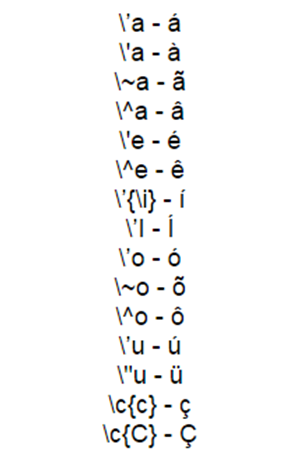
\includegraphics[scale=1.0]{Model/USPSC-img/USPSC-AcentuacaoLaTeX.png} \\
	Fonte: \citeonline{comandos}
	\end{center}	
\end{figure}

\end{anexosenv}


%---------------------------------------------------------------------
% INDICE REMISSIVO
%--------------------------------------------------------------------
% commented include
%%% USPSC-IndicexRemissivos.tex
% ---
% Inicia os Índices Remissivos
% ---
%---------------------------------------------------------------------
% INDICE REMISSIVO
%--------------------------------------------------------------------
\phantompart
\printindex
%---------------------------------------------------------------------


%---------------------------------------------------------------------

\end{document}
